\documentclass[xcolor={dvipsnames}, aspectratio=169]{beamer}
\usepackage{beamerthemesplit}
\usepackage{wrapfig}
\usetheme{SPbGU}
\usepackage{pdfpages}
\usepackage{amsmath}
\usepackage{amssymb}
\usepackage{cmap}
\usepackage[T2A]{fontenc}
\usepackage[utf8]{inputenc}
\usepackage[english]{babel}
\usepackage{indentfirst}
\usepackage{tikz}
\usetikzlibrary{shapes,arrows,arrows.meta,automata,positioning,quotes,backgrounds,decorations.text,decorations.pathmorphing}
\usepackage{multirow}
\usepackage[noend]{algpseudocode}
\usepackage{algorithm}
\usepackage{algorithmicx}
\usepackage{fancyvrb}
\usepackage[linguistics]{forest}
\usepackage{listings}
\usepackage{multicol}
\usepackage{comment}
\usepackage{xspace}
\usepackage{adjustbox}
\usepackage{makecell}
\usepackage{ stmaryrd }
\usepackage{ulem}
\usepackage{wasysym}
\usepackage{amssymb}
\usepackage{pifont}
\usepackage{animate}
\definecolor{ForestGreen}{RGB}{34,139,34}

\usepackage{xspace}
\usepackage{listings}


\newcommand{\cmark}{\textcolor{green}{\ding{51}}}
\newcommand{\xmark}{\textcolor{red}{\ding{55}}}

\newcommand{\todelete}[1]{{\color{red}{#1}}}

\newcommand{\subdued}[1]{{\color{gray}{#1}}}

\newcommand{\backupbegin}{
   \newcounter{finalframe}
   \setcounter{finalframe}{\value{framenumber}}
}
\newcommand{\backupend}{
   \setcounter{framenumber}{\value{finalframe}}
}

\newcommand{\happyCheck}{\color{green}{\checkmark}}
\newcommand{\timeout}{\color{red}{\clock}}

\newcommand{\makenote}[1]{\hfill \footnotesize{#1}}
\newcommand{\strikeoutnote}[1]{\makenote{\strikethrough{#1}}}
\newcommand{\strikethrough}[1]{\sout{#1}}

\newcommand{\lststrikethrough}[1]{\ttfamily\sout{#1}}

\newcolumntype{A}{>{\hb@xt@\z@\bgroup\hss}r<{\egroup}}
\newcolumntype{B}{>{\hb@xt@\z@\bgroup}l<{\hss\egroup}}

\setbeamertemplate{itemize item}[circle]
\setbeamertemplate{enumerate items}[circle]

\lstdefinelanguage{ocanren1}{
  basicstyle = {\ttfamily \color{black}},
  keywords=[1]{return, do, where, case, run, conde, fresh, let, match, with, when, class,
  object, method, of, rec, repeat, until, while, \begin{comment}not,\end{comment} do, done, as, val, inherit,
  new, module, sig, deriving, datatype, struct, if, then, else, open, private, virtual, include, success, failure,
  true, false, mplus},
  keywords=[2]{safe},
  keywords=[3]{unsafe},
  sensitive=true,
  commentstyle=\small\itshape\ttfamily,
  keywordstyle=[1]\color{blue},
  keywordstyle=[2]\color{ForestGreen},
  keywordstyle=[3]\color{violet},
  identifierstyle=\ttfamily,
  basewidth={0.5em,0.5em},
  columns=flexible,
  mathescape=true,
  escapechar=~,
  fontadjust=true,
  literate={fun}{{$\lambda$}}1 {function}{function}8 {->}{{$\to$}}3 {<-}{{$\leftarrow$}}3 {===}{{$\equiv$}}1 {=/=}{{$\not\equiv$}}1 {|>}{{$\triangleright$}}3 {\\/}{{$\vee$}}2 {/\\}{{$\wedge$}}2 {^}{{$\uparrow$}}1,
  morecomment=[s]{(*}{*)},
  moredelim=**[is][\color{red}]{@!}{@}
}

\lstdefinelanguage{ocanren}{
  basicstyle = {\ttfamily \color{black} \footnotesize},
  keywords=[1]{return, do, where, case, run, conde, fresh, let, match, with, when, class,
  object, method, of, rec, repeat, until, while, \begin{comment}not,\end{comment} do, done, as, val, inherit,
  new, module, sig, deriving, datatype, struct, if, then, else, open, private, virtual, include, success, failure,
  true, false, mplus, data, instance},
  backgroundcolor = {\color{Orchid!10}},
  keywords=[2]{safe},
  keywords=[3]{unsafe},
  sensitive=true,
  commentstyle=\small\itshape\ttfamily,
  keywordstyle=[1]\color{blue},
  keywordstyle=[2]\color{ForestGreen},
  keywordstyle=[3]\color{violet},
  identifierstyle=\ttfamily,
  basewidth={0.5em,0.5em},
  columns=flexible,
  mathescape=true,
  escapechar=~,
  fontadjust=true,
  literate={fun}{{$\lambda$}}1 {function}{function}8 {->}{{$\to$}}3 {<-}{{$\leftarrow$}}3 {===}{{$\equiv$}}1 {=/=}{{$\not\equiv$}}1 {\\/}{{$\vee$}}2 {/\\}{{$\wedge$}}2 {^}{{$\uparrow$}}1,
  morecomment=[s]{(*}{*)},
  moredelim=**[is][\color{red}]{@!}{@}
}

% \lstset{
%   language=ocanren
% }


\lstdefinelanguage{imperative}{
  basicstyle = {\ttfamily \color{black}},
  backgroundcolor = {\color{white}},
  keywordstyle = {\color{blue}},
  keywordstyle = [2]{\color{ForestGreen}},
  keywords = {while, do, if, then, return, procedure, for, fun, else}, 
  morekeywords = [2]{true, false, none},
}

\lstdefinelanguage{racket}{
  basicstyle = {\ttfamily \color{black} \footnotesize},
  backgroundcolor = {\color{Emerald!10}},
  keywordstyle = {\color{blue}},
  keywordstyle = [2]{\color{ForestGreen}},
  keywords = {while, do, if, then, return, procedure}, 
  morekeywords = [2]{true, false, none},
}

\lstdefinelanguage{logic}{
  basicstyle = {\ttfamily \color{black} \footnotesize},
  backgroundcolor = {\color{SkyBlue!10}},
  keywordstyle = {\color{blue}},
  keywordstyle = [2]{\color{ForestGreen}},
  keywords = {while, do, if, then, return, procedure}, 
  morekeywords = [2]{start, end},
}

\lstdefinelanguage{query}{
  basicstyle = {\ttfamily \color{black}},
  backgroundcolor = {\color{Periwinkle!10}},
  keywordstyle = {\color{blue}},
  keywordstyle = [2]{\color{ForestGreen}},
  keywords = {true, false}, 
  otherkeywords={<-,->},
  morekeywords = [2]{<-, ->, nondeterminism, predicate,ignore},
}


\lstdefinestyle{mystyle}
{
    language = C++,
    basicstyle = {\ttfamily \color{black}},
    backgroundcolor = {\color{white}},
    stringstyle = {\color{blue}},
    keywordstyle = {\color{green}},
    keywordstyle = [2]{\color{lime}},
    keywordstyle = [3]{\color{yellow}},
    keywordstyle = [4]{\color{teal}},
    otherkeywords = {;,<<,>>,++},
    morekeywords = [2]{true, false},
    morekeywords = [3]{<<, >>},
    morekeywords = [4]{++},
}

\tikzstyle{processTree} = [
  ->,
  sibling distance=15em,
  scale=0.6,
  every node/.style = {
    shape=rectangle,
    rounded corners=0.05cm,
    draw,
    align=center,
    minimum size=5mm,
    scale=0.6,},
  %level 1/.style={sibling distance=100em}
  ]


\tikzstyle{program} = [
  draw=black,
  thick,
  rectangle,
  rounded corners=1pt,
  inner sep=5pt,
  inner ysep=5pt
  ]

\tikzstyle{goal} = [
  draw=black,
  rectangle,
  rounded corners=1pt,
  inner ysep=0pt,
  ]

\tikzstyle{input} = [
  draw=none,
  rectangle,
  rounded corners=1pt,
  inner sep=2pt,
  inner ysep=2pt,
  fill=green!10,
  minimum height=5mm
  ]


\tikzstyle{transparent} = [
  draw=none,
  inner ysep=3pt
  ]



\DeclareMathOperator{\Term}{\mathcal{T}}
\DeclareMathOperator{\FlatTerm}{\mathcal{FT}}
\DeclareMathOperator{\Var}{\mathbf{Var}}
\DeclareMathOperator{\Cons}{\mathcal{C}}
\DeclareMathOperator{\Kan}{\mathcal{G}}
\DeclareMathOperator{\Fresh}{\mathbf{Fresh}}
\DeclareMathOperator{\Delay}{\mathbf{Delay}}
\DeclareMathOperator{\Cll}{\mathbf{Call}}
\DeclareMathOperator{\Def}{\mathcal{D}}
\DeclareMathOperator{\Base}{\mathbf{Base}}
\DeclareMathOperator{\Conj}{\mathbf{Conj}}
\DeclareMathOperator{\free}{\mathbf{free}}
\DeclareMathOperator{\ground}{\mathbf{ground}}
\DeclareMathOperator{\In}{\mathbf{In}}
\DeclareMathOperator{\Out}{\mathbf{Out}}
\DeclareMathOperator{\Fun}{\mathcal{F}}
\DeclareMathOperator{\Rtrn}{\mathbf{return}}
\DeclareMathOperator{\Bind}{\mathbf{Bind}}
\DeclareMathOperator{\Match}{\mathbf{Match}}
\DeclareMathOperator{\Sum}{\mathbf{<|>}}
\DeclareMathOperator{\Guard}{\mathbf{Guard}}
\DeclareMathOperator{\Gen}{\mathbf{Gen}}
\DeclareMathOperator{\Stream}{\mathit{Stream}}
\DeclareMathOperator{\vars}{vars}
\DeclareMathOperator{\inmode}{\mathtt{I}}
\DeclareMathOperator{\outmode}{\mathtt{O}}
\DeclareMathOperator{\whatmode}{\mathtt{?}}
% \DeclareMathOperator{\inmode}{g \rightarrow g}
% \DeclareMathOperator{\outmode}{f \rightarrow g}
% \DeclareMathOperator{\mode1}{mode}
% \DeclareMathOperator{\Mode1}{\mathcal{M}}
\newcommand{\KanN}{\mathcal{K}^{N}}
\newcommand{\tran}[1]{\left\llbracket #1 \right\rrbracket}
\newcommand{\LIST}[1]{ #1^*}
\renewcommand{\emptyset}{\varnothing}
\newcommand{\mk}{\textsc{miniKanren}\xspace}
\newcommand{\ocaml}{\textsc{OCaml}\xspace}
\newcommand{\haskell}{\textsc{Haskell}\xspace}
\renewcommand{\and}{$\&$\xspace}
\newcommand{\rel}[2]{\texttt{#1}$^o$ #2}
\newcommand{\subst}[1]{$\langle$#1$\rangle$}
\newcommand{\sem}[1]{\llbracket #1 \rrbracket}

\lstset{moredelim=[is][\bfseries]{[*}{*]}}

\beamertemplatenavigationsymbolsempty

\title[Relational Programming through Specialization]{Enabling Relational Programming through Specialization}
\subtitle{}
\institute[Jetbrains Research]{
JetBrains Research, Programming Lanuages and Program Analysis Lab \\
Constructor University, Bremen
}

\author[Ekaterina Verbitskaia]{Ekaterina Verbitskaia}

\date{June 5, 2024}

\definecolor{orange}{RGB}{179,36,31}

\begin{document}
{
\begin{frame}[fragile]
   \begin{center}
      
\includegraphics[height=1.5cm]{pictures/jetbrainsResearch.pdf}
    \end{center}
  \titlepage
\end{frame}
}

\begin{frame}[fragile]
  \frametitle{Find Reachable Vertices}
  \begin{columns}    
    \begin{column}{0.35\textwidth}
      \centering
      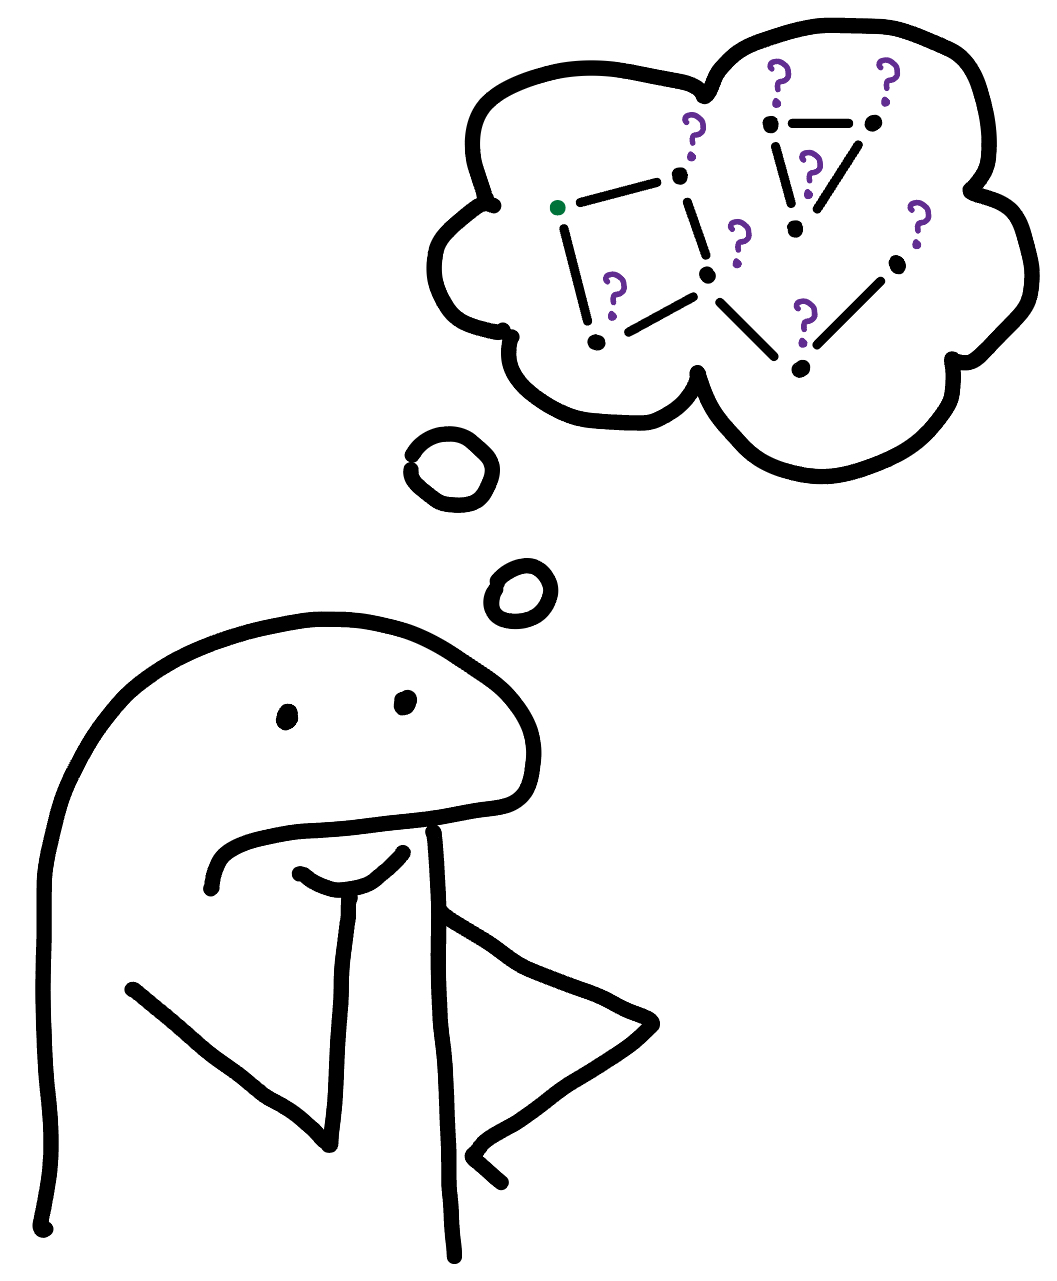
\includegraphics[width=0.8\textwidth]{pic/reachable.jpg}
    \end{column} \pause
    \begin{column}{0.75\textwidth} 
      \begin{lstlisting}[language=imperative]
    procedure DFS(G, v) = 
      S.push(v)
      while !S.empty do
        v = S.pop()
        if (!seen[v]) then
          seen.add(v)
          for (_, w) in G.edges(v) do 
            S.push(w)
          \end{lstlisting}
        \end{column}
        \end{columns}
\end{frame}


\begin{frame}[fragile]
  \frametitle{Find Reachable Vertices}
  \begin{columns}    
    \begin{column}{0.35\textwidth}
      \centering
      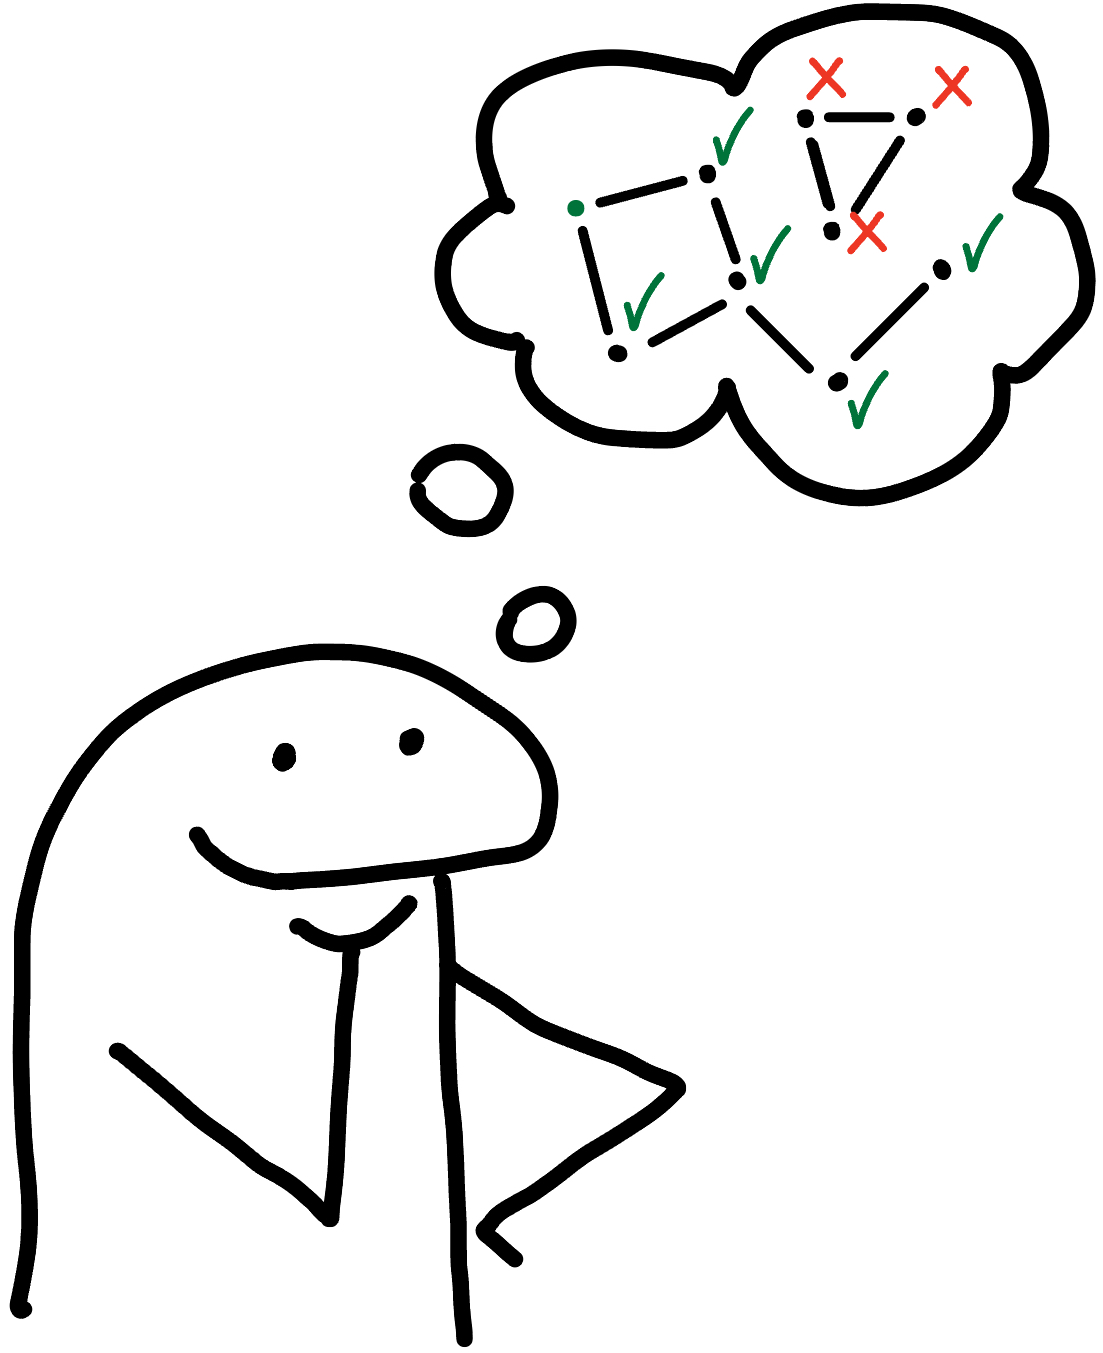
\includegraphics[width=0.8\textwidth]{pic/reachableAns.jpg}
    \end{column}
    \begin{column}{0.75\textwidth} 
      \begin{lstlisting}[language=imperative]
    procedure DFS(G, v) = 
      S.push(v)
      while !S.empty do
        v = S.pop()
        if (!seen[v]) then
          seen.add(v)
          for (_, w) in G.edges(v) do 
            S.push(w)
      \end{lstlisting}
    \end{column}
    \end{columns}
\end{frame}

\begin{frame}[fragile]
  \frametitle{Find a Path}
  \begin{columns}    
    \begin{column}{0.35\textwidth}
      \centering
      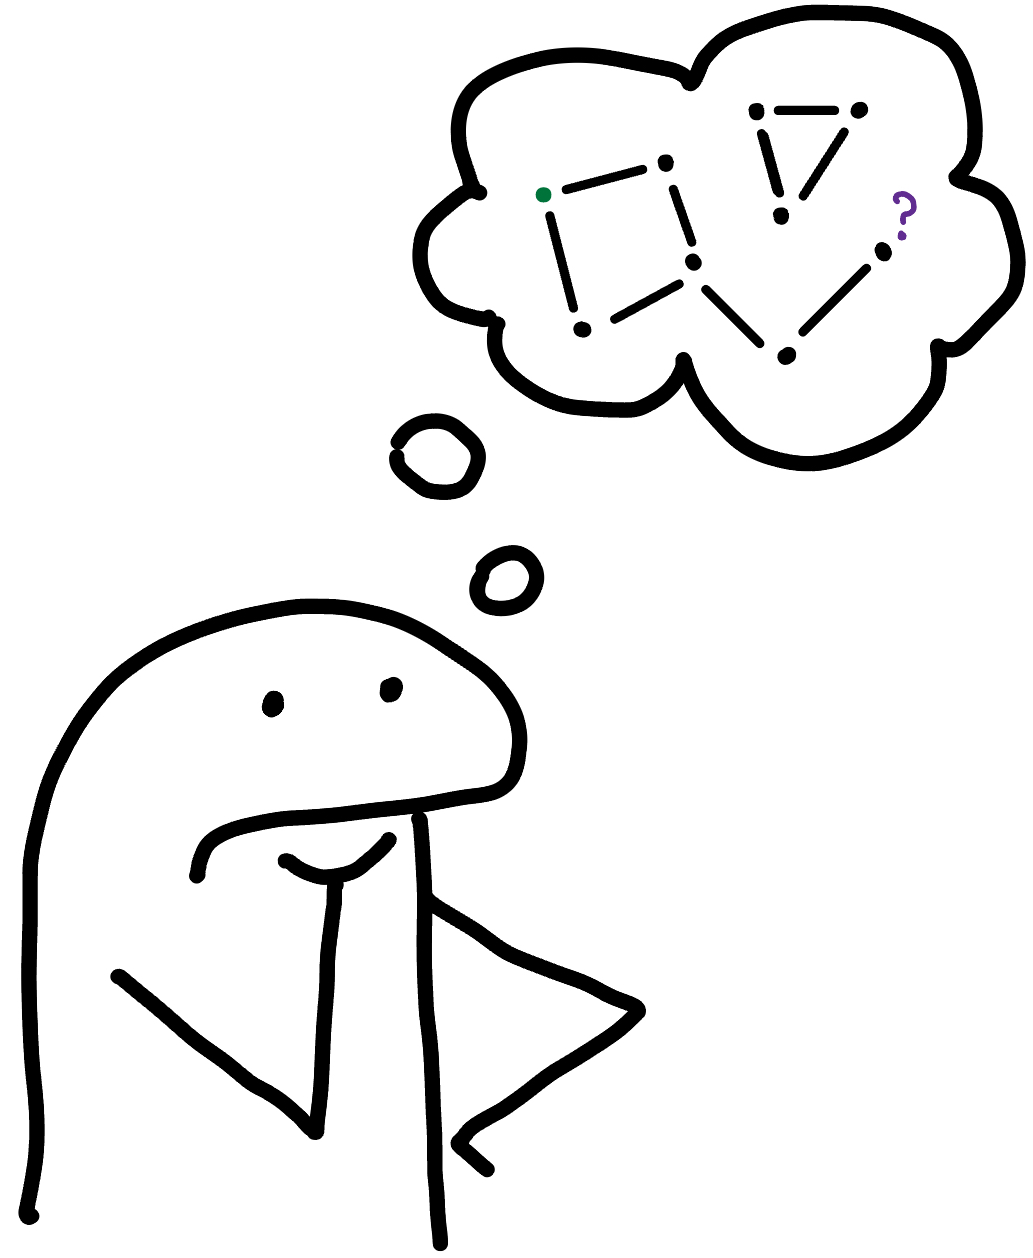
\includegraphics[width=0.8\textwidth]{pic/path.jpg}
    \end{column} \pause
    \begin{column}{0.75\textwidth} 
      \begin{lstlisting}[language=imperative]
    procedure DFS(G, v, u) = 
      S.push(v, [])
      while !S.empty do
        if (v == u) then return path
        (v, path) = S.pop()
        if (!seen[v]) then
          seen.add(v)
          for (_, w) in G.edges(v) do 
            S.push(w, path.add(w))
        return none
      \end{lstlisting}
    \end{column}
    \end{columns}
\end{frame}


\begin{frame}[fragile]
  \frametitle{Find a Path}
  \begin{columns}    
    \begin{column}{0.35\textwidth}
      \centering
      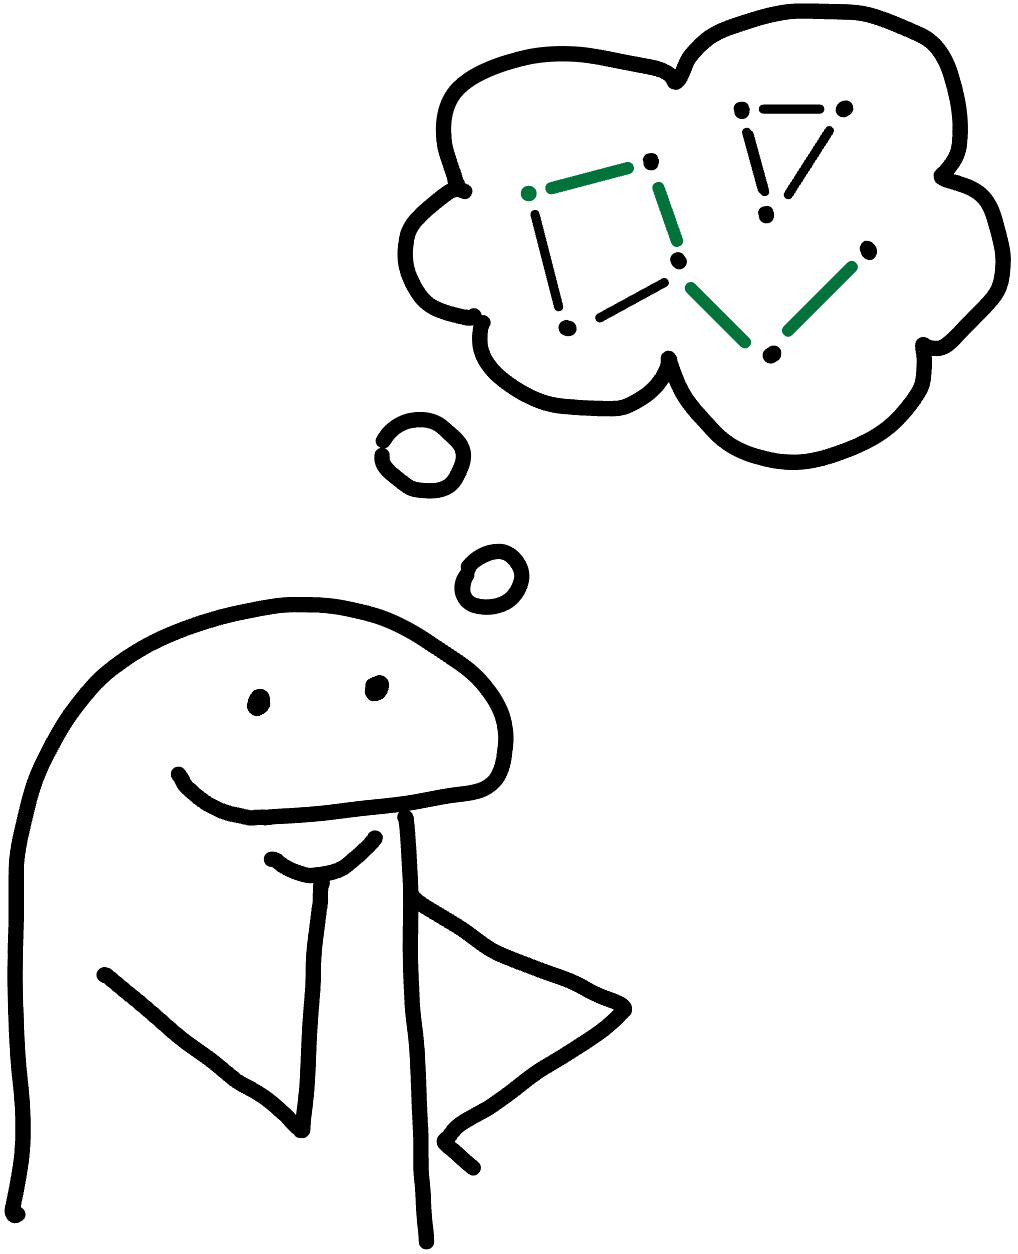
\includegraphics[width=0.8\textwidth]{pic/pathAns.jpg}
    \end{column}
    \begin{column}{0.75\textwidth} 
      \begin{lstlisting}[language=imperative]
    procedure DFS(G, v, u) = 
      S.push(v)
      path.push(v)
      while !S.empty do
        if (v == u) then return path
        v = S.pop()
        if (!seen[v]) then
          seen.add(v)
          for (_, w) in G.edges(v) do 
            S.push(w)
        path.pop()
        return none
      \end{lstlisting}
    \end{column}
    \end{columns}
\end{frame}

\begin{frame}[fragile]
  \frametitle{Find All Paths}
  \begin{columns}    
    \begin{column}{0.35\textwidth}
      \centering
      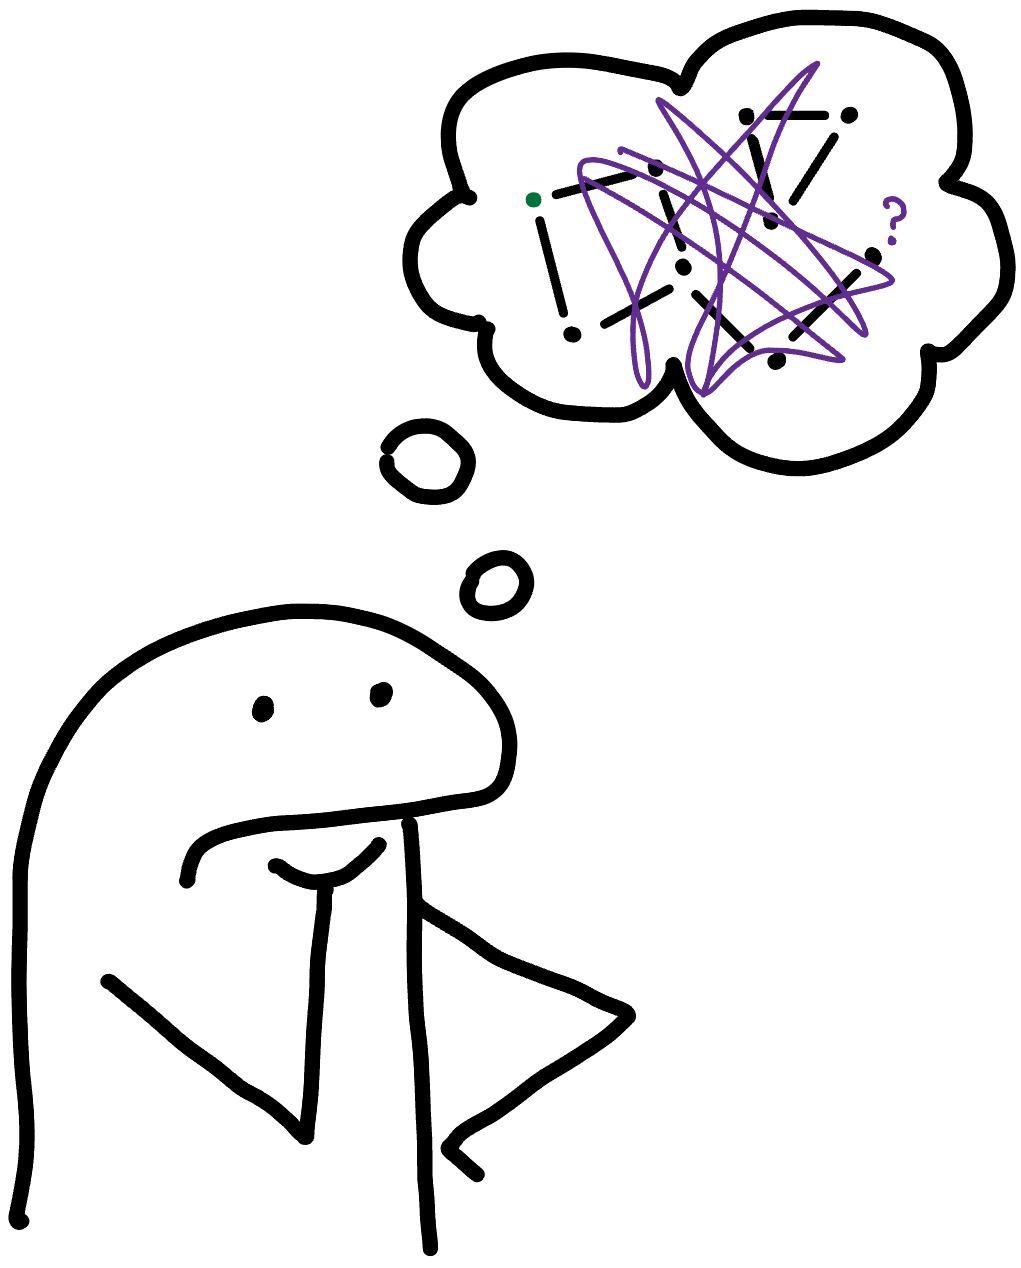
\includegraphics[width=0.8\textwidth]{pic/allPaths.jpg}
    \end{column}
    \begin{column}{0.75\textwidth} 
      \begin{lstlisting}[language=imperative]

      \end{lstlisting}
    \end{column}
    \end{columns}
\end{frame}

\begin{frame}[fragile]
  \frametitle{What is a Path?}
  \begin{columns}    
    \begin{column}{0.35\textwidth}
      \centering
      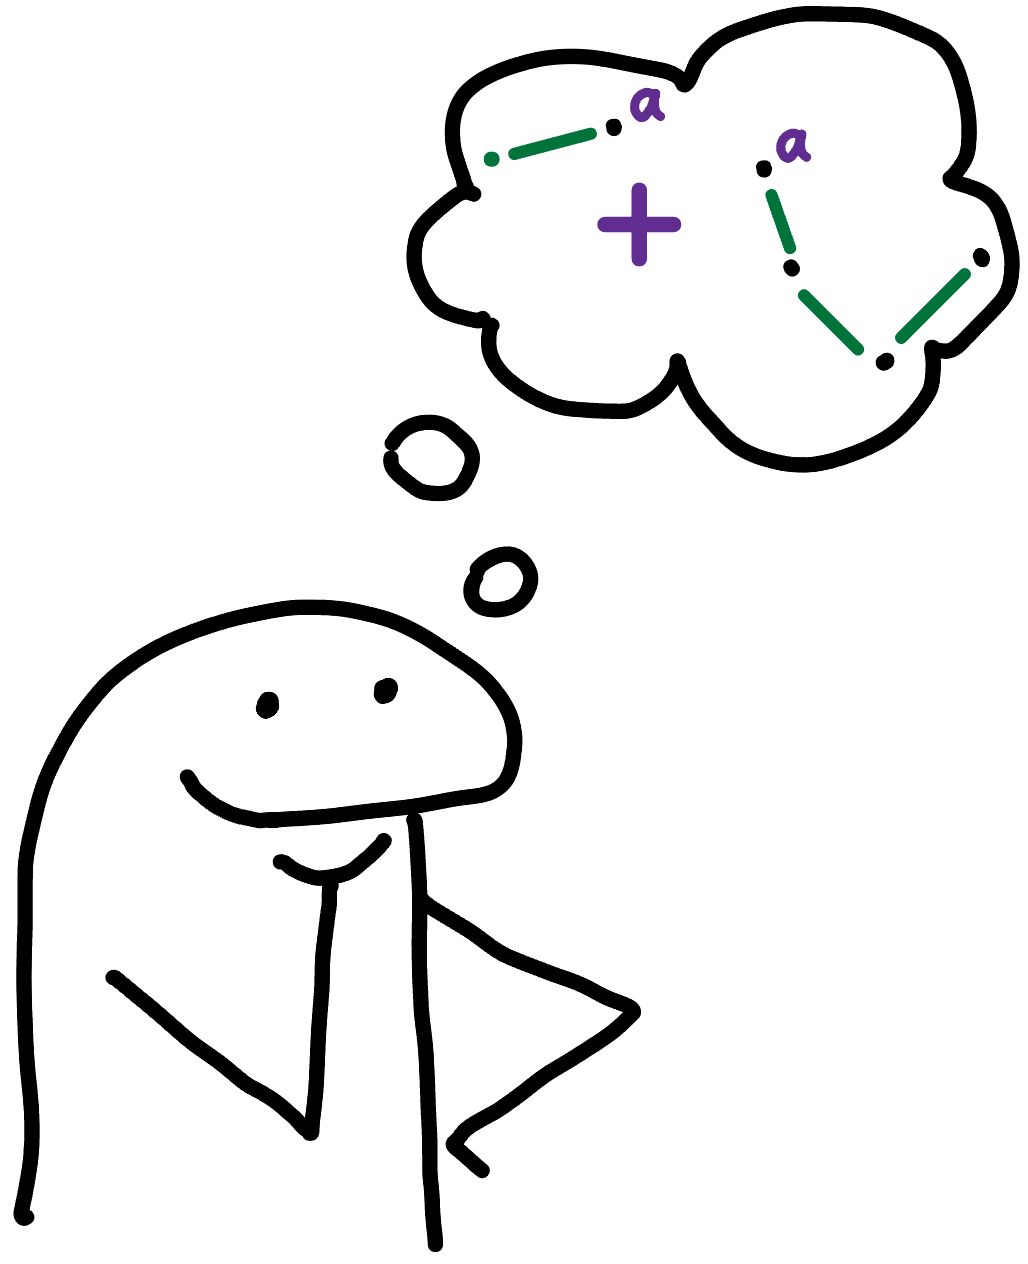
\includegraphics[width=0.8\textwidth]{pic/pathIs.jpg}
    \end{column}
    \begin{column}{0.75\textwidth} 
\[
\begin{array}{rcl}
  path(v, u) &=& [v], if \, v = u \\ 
             &|& \exists w: edge(v, w) \wedge path(w, u)
\end{array}
\]

\pause 

\begin{center}
  \begin{minipage}{0.82\textwidth}
    \begin{lstlisting}[language=logic,escapechar=@]
path(V, V, [V]). 
path(V, U, [V|P]) :- edge(V, W), path(W, U, P).
     @\color{ForestGreen}{|}@  @\color{ForestGreen}{|}@    @\color{ForestGreen}{|}@
 start  end  @\color{ForestGreen}{path}@                      % Prolog
    \end{lstlisting}
  \end{minipage}  
\end{center}
    \end{column}
    \end{columns}
\end{frame}


\begin{frame}[fragile]
  \frametitle{Logic Programming: Querying Paths}
  \begin{columns}    
    \begin{column}{0.35\textwidth}
      \centering
      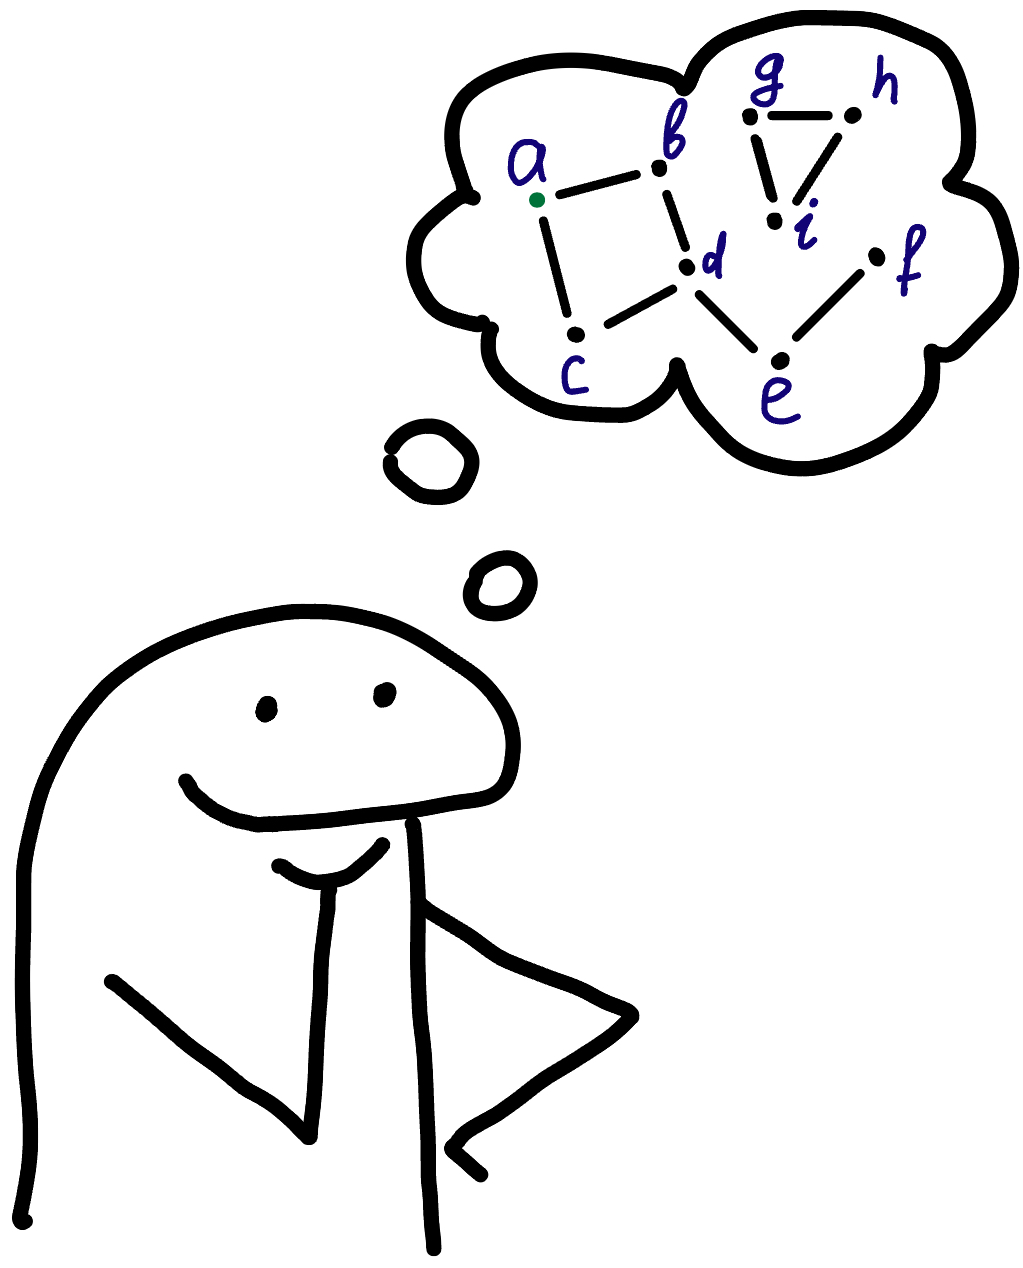
\includegraphics[width=0.8\textwidth]{pic/graph.jpg}
    \end{column}
    \begin{column}{0.75\textwidth} 

\begin{center}
  \begin{minipage}{0.82\textwidth}
    \begin{lstlisting}[language=logic]
edge(a, b).
edge(a, c).
...
edge(i, g).

path(V, V, [V]). 
path(V, U, [V|P]) :- edge(V, W), path(W, U, P).
    \end{lstlisting}

    \begin{lstlisting}[language=query,basicstyle=\footnotesize]
? path(a, f, _).             ? path(a, h, _).
true     <- predicate ->     false 
                              
? path(a, f, P).              

P = [a, b, d, e, f]      
P = [a, c, d, e, f]      <- nondeterminism
false 
    \end{lstlisting}
  \end{minipage}
\end{center}

      \end{column}
    \end{columns}
\end{frame}


\begin{frame}[fragile]
  \frametitle{Logic Programming: Querying Reachable Vertices}
  \begin{columns}    
    \begin{column}{0.35\textwidth}
      \centering
      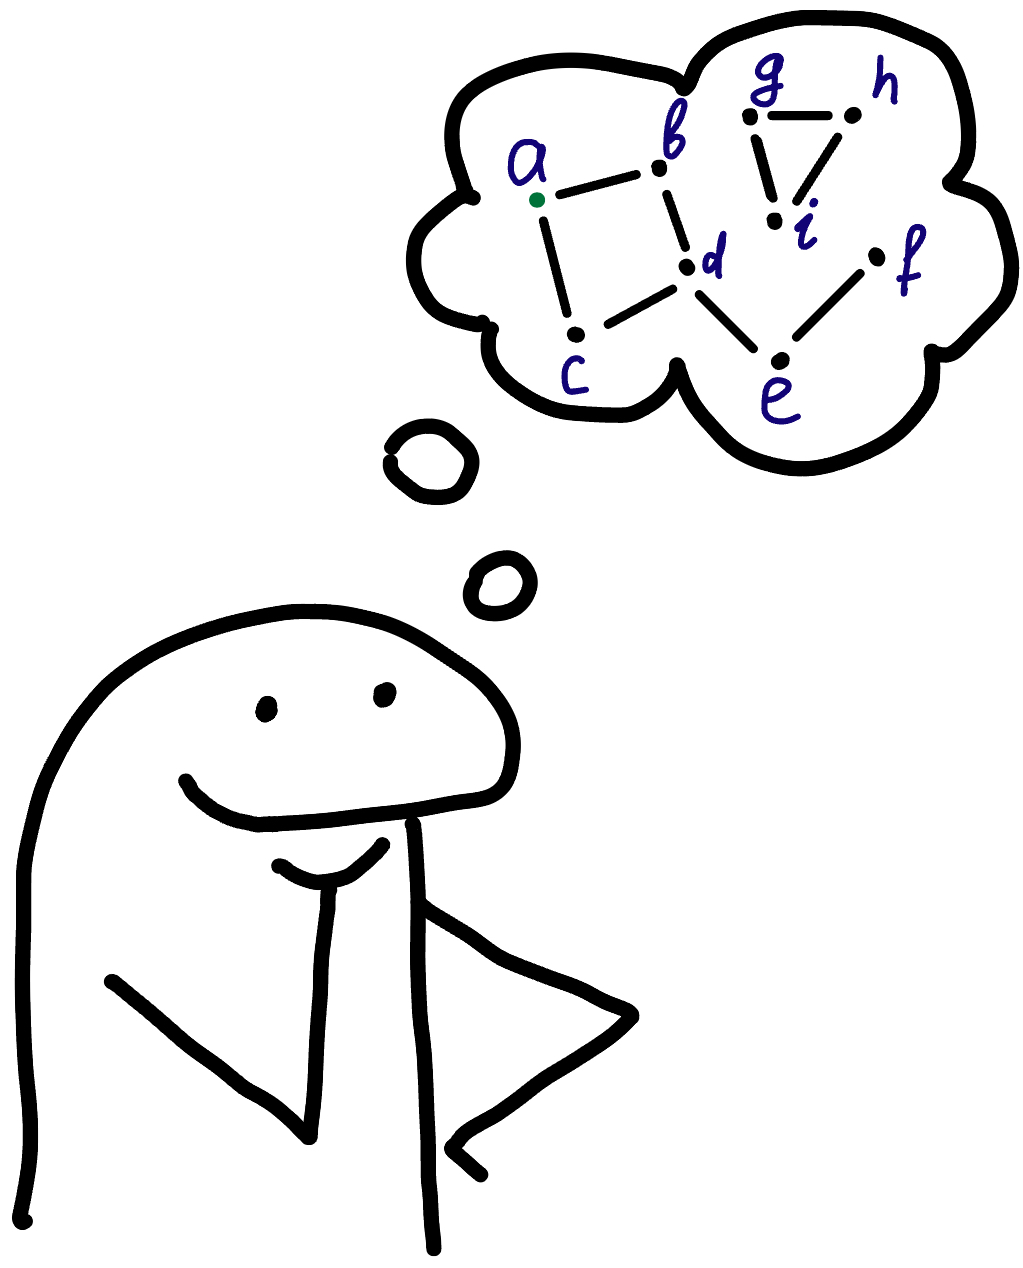
\includegraphics[width=0.8\textwidth]{pic/graph.jpg}
    \end{column}
    \begin{column}{0.75\textwidth}       
\begin{center}
  \begin{minipage}{0.82\textwidth}
    \begin{lstlisting}[language=logic]
edge(a, b).
edge(a, c).
...
edge(i, g).

path(V, V, [V]). 
path(V, U, [V|P]) :- edge(V, W), path(W, U, P).
    \end{lstlisting}

    \begin{lstlisting}[language=query,basicstyle=\footnotesize,escapechar=@]
? path(a, X, _).
             @\color{ForestGreen}{|}@ 
X = a        ignore
X = b 
X = d 
X = e
X = f 
false 
    \end{lstlisting}
  \end{minipage}
\end{center}

      \end{column}
    \end{columns}
\end{frame}

\begin{frame}[fragile]
  \frametitle{Relational Programming in \mk}

  \begin{columns}    
    \begin{column}{0.35\textwidth}
      \centering
      
\includegraphics[width=0.8\textwidth]{pic/edsl.jpg}
    \end{column}
    \begin{column}{0.75\textwidth}       
\begin{center}
  \begin{minipage}{0.82\textwidth}
    \begin{lstlisting}[language=racket]
(define (patho v u p)                 ; Racket
  (fresh (w p1)
    (conde
      [(== v u) (== p `(,v))]
      [(edge v w)
       (patho w u p1)
       (== p (cons v p1))])))

(run* (q) (patho 'a 'e q))
    \end{lstlisting}

    \begin{lstlisting}[language=ocanren]
 let rec path$^o$ v u p =                      (* OCaml *)
   (v === u /\ p === [v]) \/
   (fresh (w p$_1$)
     (edge$^o$ v w /\
       path$^o$ w$_1$ u p$_1$ /\
       p === v : p$_1$) )
         \end{lstlisting}
  \end{minipage}
\end{center}

      \end{column}
    \end{columns}
\end{frame}

\begin{frame}[fragile]
  \frametitle{}

\begin{center}
  \Large \mk
\end{center}

\end{frame}

\begin{frame}[fragile]
  \frametitle{The Anatomy of \mk}

\begin{center}
\begin{tikzpicture}[
  every node/.style = {
    shape=rectangle,
    rounded corners=0.05cm,
    draw,
    align=center,
    minimum size=5mm},
  node distance=1.3em,
  anchor=center
]
  \node[inner sep=10pt,draw=none] (code) at (0,-1) {\begin{lstlisting}[language=ocanren,basicstyle=\ttfamily,backgroundcolor=\color{white}]
let rec path$^o$ v u p = 
  (v === u /\ p === []) \/
  (fresh (w p$_1$)
    (edge$^o$ v w /\
     path$^o$ w$_1$ u p$_1$ /\
     p === v : p$_1$) )
    \end{lstlisting}};
    \node (rel) [draw=none, right=of code, yshift=1.5cm] {relation};
    \draw [teal,<-] ($(code.north)+(-0.2,-0.45)$) to [out=60,in=180] node[below, draw=none, teal] {} ($(rel.west)+(0,-0.1)$);
    
    \pause
    \node (call) [draw=none, left=of code, yshift=-1.5cm] {relation call};
    \draw [teal,<-] ($(code.south)+(-1.3,1.5)$) to [out=-180,in=45] node[below, draw=none, teal] {} ($(call.east)+(0,0)$);
    \draw [teal,<-] ($(code.south)+(-1.3,1.1)$) to [out=-180,in=45] node[below, draw=none, teal] {} ($(call.east)+(0,0)$);
    
    \pause
    \node (uni) [draw=none, left=of code, yshift=1.5cm] {term unification};
    \draw [teal,<-] ($(code.west)+(1.4,0.75)$) to [out=150,in=-45] node[below, draw=none, teal] {} ($(uni.east)+(0,-0.1)$);
    
    \pause
    \node (conj) [draw=none, right=of code, yshift=-1.5cm] {conjunction};
    \draw [teal,<-] ($(code.east)+(-0.7,-0.75)$) to [out=2,in=120] node[below, draw=none, teal] {} ($(conj.west)+(0,0)$);
    \draw [teal,<-] ($(code.east)+(-1.4,-0.25)$) to [out=0,in=120] node[below, draw=none, teal] {} ($(conj.west)+(0,0)$);
    
    \pause
    \node (disj) [draw=none, right=of code, yshift=0cm] {disjunction};
    \draw [teal,<-] ($(code.east)+(-0.4,0.7)$) to [out=0,in=180] node[below, draw=none, teal] {} ($(disj.west)+(0,0)$);
    
    \pause
    \node (fresh) [draw=none, left=of code, yshift=0cm] {variable introduction};
    \draw [teal,<-] ($(code.west)+(0.7,0.15)$) to [out=180,in=0] node[below, draw=none, teal] {} ($(fresh.east)+(0,0)$);
\end{tikzpicture}
\end{center}


\end{frame}

\begin{frame}[fragile]
  \frametitle{The Semantics of \mk: Unification}

\begin{columns}
  \begin{column}{0.45\textwidth}
    \[ f(x, A, g(z), y) \equiv f(h(A, y), A, g(B), y)\] 
  
    \vspace{-0.4cm}
  
    \[ \{x \mapsto h(A, y), z \mapsto B \} \]
  
    \vspace{0.8cm}
  
    \[ f(x, x) \equiv f(h(A, y), g(B))\] 

    \vspace{-0.4cm}

    \[ \emptyset \]
  
  \end{column}
  
  \begin{column}{0.45\textwidth}

    \begin{lstlisting}[language=ocanren]
 (===) :: Term -> Term -> Subst -> Subst 
    \end{lstlisting}
  \end{column}
\end{columns}

\end{frame}

\begin{frame}[fragile]
  \frametitle{The Semantics of \mk: Stream}
    \begin{lstlisting}[language=ocanren]
data Stream a = Empty | Mature a (Stream a) 

instance Alternative Stream where
  empty = Empty

  (Mature h tl) <|> y = Mature h (y <|> tl)
  Empty         <|> y = y

instance Monad Stream where
  Empty >>= _ = mzero
  Mature x xs >>= g = mplus (g x) (xs >>= g)

(/\) = (>>=)
(\/) = (<|>)
    \end{lstlisting} 
\end{frame}

\begin{frame}[fragile]
  \frametitle{}

\begin{center}
  \Large Solvers from Verifiers
\end{center}

\end{frame}

\begin{frame}[fragile]
  \frametitle{Verifiers}
  \begin{columns}    
    \begin{column}{0.35\textwidth}
      \centering
      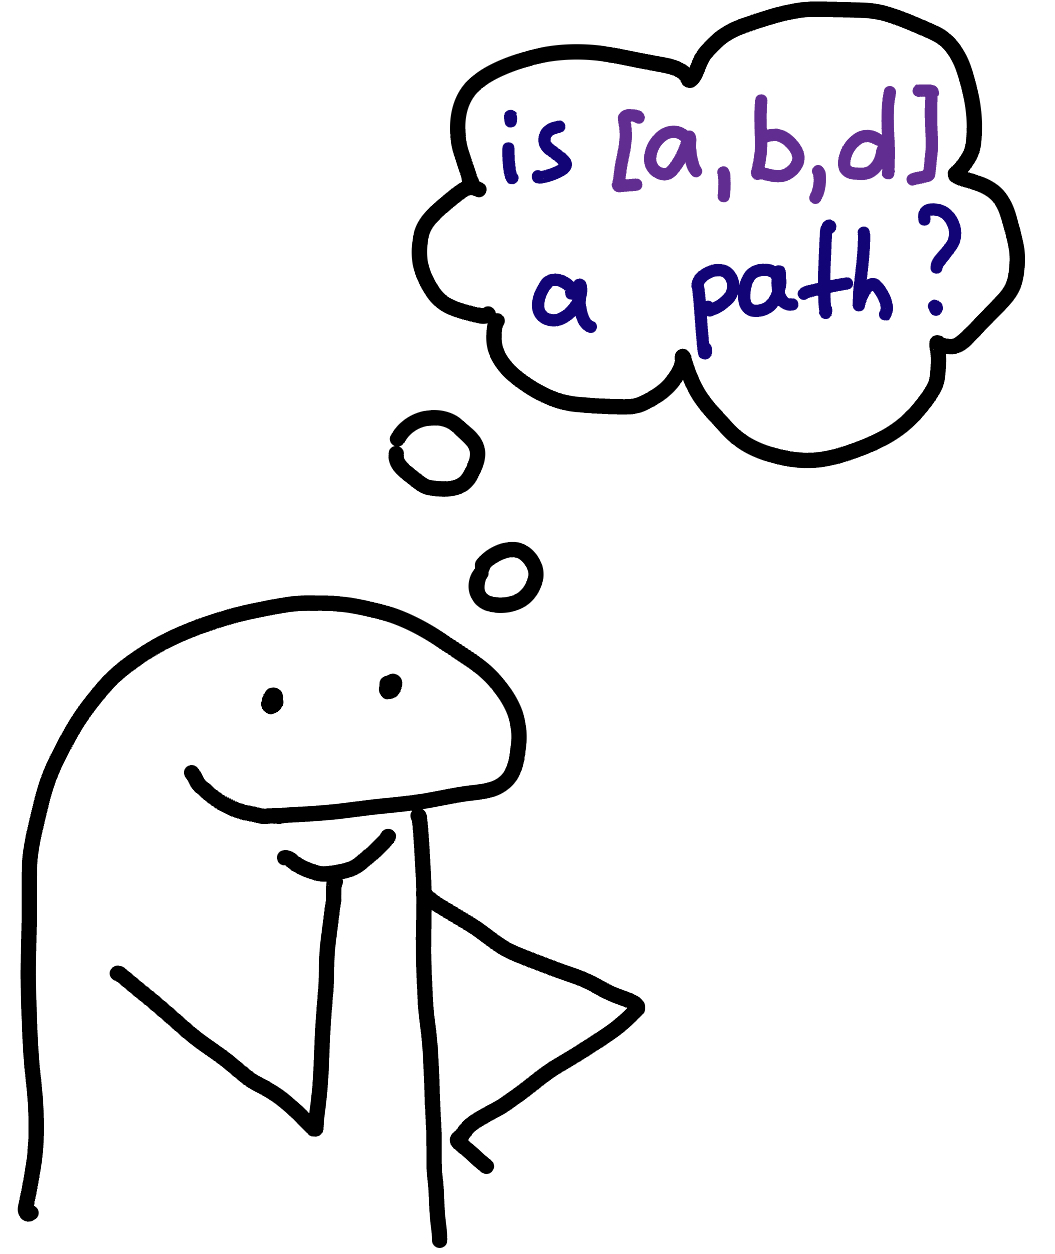
\includegraphics[width=0.8\textwidth]{pic/verifier.jpg}
    \end{column}
    \begin{column}{0.75\textwidth} 
      \begin{center}
        \begin{minipage}{0.82\textwidth}
      \begin{lstlisting}[language=ocanren]
  let rec is_path path =
    match path with 
    | [], [_] -> true 
    | u :: v :: t -> 
        if edge u v 
        then is_path (v :: t)
        else false 
      \end{lstlisting}
    \end{minipage}
  \end{center}      
    \end{column}
  \end{columns}
\end{frame}


\begin{frame}[fragile]
  \frametitle{Solvers}
  \begin{columns}    
    \begin{column}{0.35\textwidth}
      \centering
      
\includegraphics[width=0.8\textwidth]{pic/solver.jpg}
    \end{column}
    \begin{column}{0.75\textwidth} 
      \begin{center}
        \begin{minipage}{0.82\textwidth}
      \begin{lstlisting}[language=ocanren]
  let rec dfs ... = 
    push stack ... 
    while ...
      ... pop stack 
      if seen ...
        ... dfs ...  
      ... return ... 
      \end{lstlisting}
    \end{minipage}
  \end{center}      
    \end{column}
  \end{columns}
\end{frame}

\begin{frame}[fragile]
  \frametitle{Solvers from Verifiers}
  \begin{columns}    
    \begin{column}{0.35\textwidth}
      \centering
      
\includegraphics[width=0.8\textwidth]{pic/kanren.jpg}
    \end{column}
    \begin{column}{0.75\textwidth} 
\begin{center}
\begin{tikzpicture}[
  every node/.style = {
    shape=rectangle,
    rounded corners=0.05cm,
    draw,
    align=center,
    minimum size=5mm},
  node distance=1.3em,
  anchor=center
]

\node[inner sep=10pt,draw=none] (function) at (0,0) {
\begin{minipage}{0.82\textwidth}
\begin{lstlisting}[language=ocanren]
 let rec is_path path =                 (* function *)
   match path with 
   | [], [_] -> true 
   | u :: v :: t -> 
       if edge u v 
       then is_path (v :: t)
       else false 
\end{lstlisting}
\end{minipage}}; 

\node[inner sep=10pt,draw=none] (relation) at (0,-3.5) {
\begin{minipage}{0.82\textwidth}
\begin{lstlisting}[language=ocanren]
 let rec path$^o$ v u p =     (* relational interpreter*)
   (v === u /\ p === [v]) \/
   (fresh (w p$_1$)
     (edge$^o$ v w /\
      path$^o$ w$_1$ u p$_1$ /\
      p === v : p$_1$) )
\end{lstlisting}
\end{minipage}}; 

  \node (unnesting) at ($(relation.north)!0.5!(function.south)$) [draw=none, xshift=-0.1cm] {relational conversion};
  \draw [teal,thick,->] ($(function.south)+(-2,0.5)$) to [out=-90,in=90] ($(relation.north)+(-2,-0.5)$);

  \node (verifier) at ($(relation.center)$) [draw=none, xshift=2cm, yshift=0.5cm,anchor=west] {verifier};
  \draw [teal,thick,->] ($(relation.center)+(-0.5,0)$) to [out=0,in=180] ($(verifier.west)+(0,0)$);

  \node (solver) at ($(relation.center)$) [draw=none, xshift=2cm, yshift=-0.5cm,anchor=west] {solver};
  \draw [teal,thick,->] ($(relation.center)+(-0.5,0)$) to [out=0,in=180] ($(solver.west)+(0,0)$);
  \end{tikzpicture}
\end{center}

    \end{column}
  \end{columns} 
\end{frame}

\begin{frame}[fragile]
  \frametitle{Solvers from Verifiers: Examples}
  \begin{columns}    
    \begin{column}{0.35\textwidth}
      \centering
      
\includegraphics[width=0.8\textwidth]{pic/kanren.jpg}
    \end{column}
    \begin{column}{0.75\textwidth} 
\begin{center}
\begin{tikzpicture}[
  every node/.style = {
    shape=rectangle,
    rounded corners=0.05cm,
    draw,
    align=center,
    minimum size=5mm},
  node distance=1.3em,
  anchor=center
]

\node[draw=none] (evalo) at (0,0) {
\begin{minipage}{0.82\textwidth}
\begin{lstlisting}[language=ocanren]
 let rec eval$^o$ st fm u = 
   fresh (x y v w z) 
     (fm === Conj x y /\
      eval$^o$ st x v /\
      eval$^o$ st y w /\
      and$^o$ v w u) \/
      ... 
\end{lstlisting}
\end{minipage}}; 

\node[draw=none] (typeo) at (0,-3.5) {
\begin{minipage}{0.82\textwidth}
\begin{lstlisting}[language=ocanren]
 let rec type$^o$ e t = 
   (fresh (x y)
     (e === Int x /\ t = TInt) \/
     (e === Plus x y /\
      type$^o$ x Int /\
      type$^o$ y Int /\ 
      t === Int)) \/
      ...  
\end{lstlisting}
\end{minipage}}; 

  \node (evaluation) at ($(evalo.center)$) [draw=none, xshift=1.4cm, yshift=0.5cm,anchor=west] {evaluation};
  \draw [teal,thick,->] ($(evalo.center)+(0,0)$) to [out=0,in=180] ($(evaluation.west)+(0,0)$);

  \node (generation) at ($(evalo.center)$) [draw=none, xshift=1.4cm, yshift=-0.5cm,anchor=west] {program generation};
  \draw [teal,thick,->] ($(evalo.center)+(0,0)$) to [out=0,in=180] ($(generation.west)+(0,0)$);


  \node (typeCheck) at ($(typeo.center)$) [draw=none, xshift=1.4cm, yshift=1cm,anchor=west] {type checking};
  \draw [teal,thick,->] ($(typeo.center)+(0,0)$) to [out=0,in=180] ($(typeCheck.west)+(0,0)$);

  \node (typeInf) at ($(typeo.center)$) [draw=none, xshift=1.4cm, yshift=0cm,anchor=west] {type inference};
  \draw [teal,thick,->] ($(typeo.center)+(0,0)$) to [out=0,in=180] ($(typeInf.west)+(0,0)$);

  \node (typeInh) at ($(typeo.center)$) [draw=none, xshift=1.4cm, yshift=-1cm,anchor=west] {type inhabitance};
  \draw [teal,thick,->] ($(typeo.center)+(0,0)$) to [out=0,in=180] ($(typeInh.west)+(0,0)$);
  \end{tikzpicture}
\end{center}

    \end{column}
  \end{columns}
\end{frame}


\begin{frame}[fragile]
  \frametitle{The Issue}
  \begin{columns}    
    \begin{column}{0.35\textwidth}
      \centering
      
\includegraphics[width=0.8\textwidth]{pic/slow.jpg}
    \end{column} \pause
    \begin{column}{0.75\textwidth} 
    \begin{itemize}
      \item Unifications are expensive
      \item The order of conjunctions is finicky
      \item But! We know something that can help
    \end{itemize}
    \end{column}
  \end{columns}

\end{frame}

\begin{frame}[fragile]
  \frametitle{}

\begin{center}
  \Large Specialization
\end{center}

\end{frame}


\begin{frame}[fragile]
  \frametitle{Specialization}

  \begin{columns}    
    \begin{column}{0.35\textwidth}
      \centering
      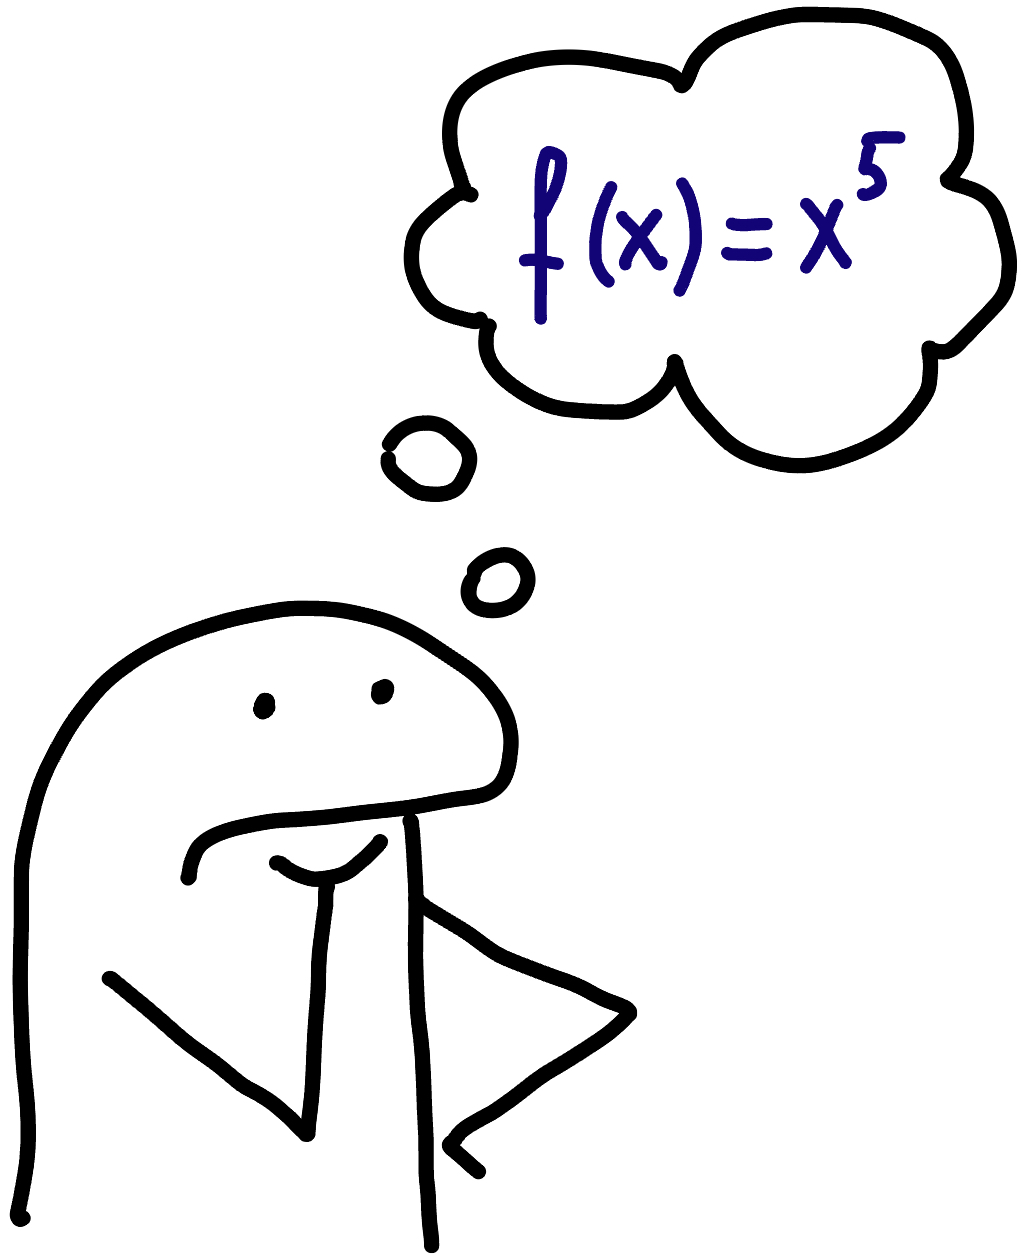
\includegraphics[width=0.8\textwidth]{pic/power.jpg}
    \end{column}
    \begin{column}{0.75\textwidth} 
      \begin{lstlisting}[language=ocanren]
 let rec power base exp = 
   if exp == 0 
   then 1 
   else base * power base (exp - 1)
          \end{lstlisting}

          \begin{lstlisting}[language=ocanren]
 let rec power_5 base =                    (* power base 5 *)
   base * base * base * base * base 
           \end{lstlisting}
        \end{column}
        \end{columns}

\end{frame}

\begin{frame}[fragile]
  \frametitle{Specialization}

  \begin{columns}    
    \begin{column}{0.35\textwidth}
      \centering
      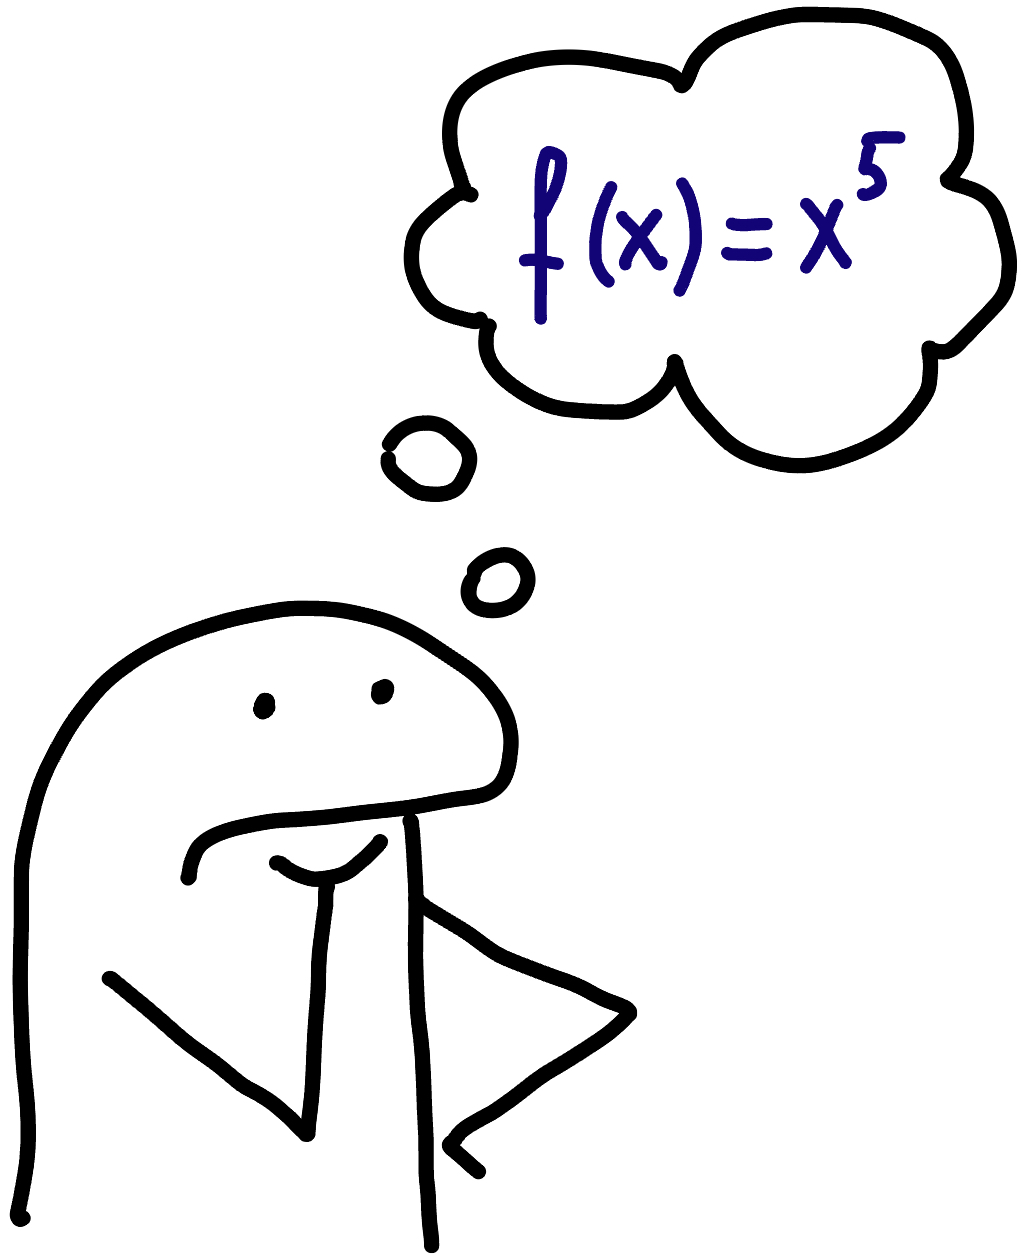
\includegraphics[width=0.8\textwidth]{pic/power.jpg}
    \end{column}
    \begin{column}{0.75\textwidth} 
\[
  program: I_{static} \times I_{dynamic} \to O 
\]

\[
  program_{I_{static}}: I_{dynamic} \to O 
\]

\vspace{0.5cm}

\begin{center}
  Same outputs for the same inputs
\end{center}
        \end{column}
        \end{columns}

\end{frame}

\begin{frame}[fragile]
  \frametitle{Specialization for \mk}
\lstset{language=ocanren1}
\begin{tikzpicture}[
  node distance = 10mm and 11 mm,
  decoration = {
    snake,
    pre length=2pt,
    post length=2pt
  },
  remember picture,
  overlay]
  \node (a) [
    program,
    anchor=north west,
    xshift=0.4cm,
    yshift=-1.1cm]
  at (current page.north west)
  {
    \adjustbox{scale=0.7}{
      \begin{minipage}[c]{0.63\textwidth}
        \begin{lstlisting}
let rec eval$^o$ fm s r =
  fm === neg x /\ not$^o$ a r /\ eval$^o$ x s a \/
  ...
        \end{lstlisting}
      \end{minipage}
    }
  };

  \node [transparent,anchor=north east] at (a.north east) {
    \footnotesize
    input program
  };

  \pause

  \node (c) [goal,anchor=north east] at (a.south east)
  {
    \adjustbox{scale=0.7}{
      \begin{minipage}[c]{0.25\textwidth}
        \begin{lstlisting}
eval$^o$ fm s true
        \end{lstlisting}
      \end{minipage}
    }
  };

  \node (lbl) [transparent,anchor=south west] at (a.south east) {
    \footnotesize
    known argument
  };

  \draw [dashed,->] (lbl.south) to [out=270,in=0] ($(c.east)-(0.7,0)$);
  \pause

  \node (d) [input, below=of a]
  {
    \adjustbox{scale=0.7}{
      \begin{minipage}[c]{0.65\textwidth}
        \begin{lstlisting}
fm === neg x /\ not$^o$ a true /\ eval$^o$ x s a \/
...
        \end{lstlisting}
      \end{minipage}
    }
  };

  \path[draw=black,->,thick, decorate] (a.south) to (d.north);

  \pause

  \node (e) [input, below=of d]
  {
    \adjustbox{scale=0.7}{
      \begin{minipage}[c]{0.5\textwidth}
        \begin{lstlisting}
fm === neg x /\ eval$^o$ x s false \/
...
        \end{lstlisting}
      \end{minipage}
    }
  };

  \path[draw=black,->,thick, decorate] (d.south) to (e.north);

  \pause

  \node (dots) [input, below=of e] {...};

  \path[draw=black,->,thick, decorate] (e.south) to (dots.north);

  \pause

  \node (b) [
    program,
    anchor=south east,
    xshift=-0.4cm,
    yshift=0.7cm]
  at (current page.south east)
  {
    \adjustbox{scale=0.7}{
      \begin{minipage}[c]{0.53\textwidth}
        \begin{lstlisting}
let rec eval_true$^o$ fm s =
  fm === neg x /\ eval_false$^o$ x s \/
  ...

let rec eval_false$^o$ fm s =
  fm === neg x /\ eval_true$^o$ x s \/
  ...
        \end{lstlisting}
      \end{minipage}
    }
  };

  \node [transparent,anchor=north east] at (b.north east) {
    \footnotesize
    output
  };
\onslide<1->
\end{tikzpicture}

\end{frame}



\begin{frame}[fragile]
  \frametitle{Specialization for \mk: Bird's Eye View}
\lstset{language=ocanren1}
\begin{tikzpicture}[
  node distance = 14mm and 13 mm,
  decoration = {
    snake,
    pre length=2pt,
    post length=4pt,
    amplitude=0.5pt,
    segment length=4pt
  },
  remember picture,overlay]
  \node (a) [
    program,
    anchor=north west,
    xshift=1cm,
    yshift=-1.3cm]
  at (current page.north west)
  {
    \adjustbox{scale=0.65}{
      \begin{minipage}[c]{0.38\textwidth}
        \begin{lstlisting}
let rec eval$^o$ fm s r =
  ...
  fm === conj x y /\
  and$^o$ a b r /\
  eval$^o$ x s a /\
  eval$^o$ y s b \/
  ...
        \end{lstlisting}
      \end{minipage}
    }
  };

  \node (b) [goal,anchor=north east] at (a.south east)
  {
    \adjustbox{scale=0.65}{
      \begin{minipage}[c]{0.24\textwidth}
        \begin{lstlisting}
eval$^o$ fm s true
        \end{lstlisting}
      \end{minipage}
    }
  };

  \pause

  \node (d) [
    transparent,
    xshift=-1cm,
    yshift=-1.3cm,
    anchor=north east]
  at (current page.north east)
  {
      \begin{tikzpicture}[
  processTree,
  sibling distance=7em,
  level distance=7em,
  level 2/.style={level distance=5em},
  anchor=center]
  \node {
    \rel{eval}{$fm \ s \ true$}}
    child { node[draw=none, fill=none] {...}}
    child { node {
      \rel{and}{$a \ b \ true$} $\wedge$  \\
      \rel{eval}{$x \ s \ a$} $\wedge$ \\
      \rel{eval}{$y \ s \ b$} \\
      \subst{$fm \to conj \ x \ y$}} 
      child { node[draw=none, fill=none] {...}}
      }
    child { node[draw=none, fill=none] {...}}
  ;
\end{tikzpicture}
  };

  \draw[->,semithick, decorate]
    ($(a.north east)+(0,-1)$) to
    [out=15,in=165,"{\footnotesize driving}"]
    ($(d.north west)+(0,-1)$);

  \pause

  \node (e) [transparent, anchor=north] at ($(d.north)+(0.3,-4.3)$)
  {
    \begin{minipage}[c]{0.4\textwidth}
      \begin{tikzpicture}[
  processTree,
  sibling distance=4em,
  level distance=3em,
  level 3/.style={level distance=4em,sibling distance=8em},
  anchor=center]
  \node (root) {
    \rel{eval}{$fm \ s \ true$}}
    child { node[draw=none, fill=none] {...}}
    child { node[draw=none, fill=none] {...}
      child { node {
        \rel{eval}{$x \ s \ true$} $\wedge$ \\
        \rel{eval}{$y \ s \ true$}}
        child { node (1) {\rel{eval}{$x \ s \ true$}}}
        child { node (2) {\rel{eval}{$y \ s \ true$}}}
        }
    }
    child { node[draw=none, fill=none] {...}}
  ;

  \draw [dashed,->] (1.west) to [out=170,in=-150] (root.west);
  \draw [dashed,->] (2.east) to [out=10,in=-30] (root.east);


\end{tikzpicture}
    \end{minipage}
  };

  \draw[->,semithick, decorate]
    ($(d.south)+(0.5,0.3)$) to
    [out=-75,in=75,"{\footnotesize folding}"]
    ($(e.north)+(0.2,0)$);

  \pause

  \node (c) [
    program,
    anchor=south west,
    xshift=1cm,
    yshift=0.8cm]
  at (current page.south west)
  {
    \adjustbox{scale=0.65}{
      \begin{minipage}[c]{0.4\textwidth}
        \begin{lstlisting}
let rec eval$^o$_true fm s =
  ...
  fm === conj x y /\
  eval$^o$_true x s /\
  eval$^o$_true y s \/
  ...
        \end{lstlisting}
      \end{minipage}
    }
  };

  \draw[->,semithick, decorate]
    ($(e.west)+(0.45,0)$) to
    [out=200,in=-20,"{\footnotesize residualization}",pos=0.5]
    (c.east);

    \onslide<1->
\end{tikzpicture}
\end{frame}

\begin{frame}[fragile]
  \frametitle{Specialization for \mk: ConsPD}
  \begin{center}
    \begin{minipage}{0.8\textwidth}
      \begin{tikzpicture}[
  processTree,
  level 1/.style={sibling distance=21em, level distance=7em},
  level 2/.style={sibling distance=10em},
  level 3/.style={level distance=6em},
  level 4/.style={level distance=4em},
  level 5/.style={sibling distance=2em, level distance=4em},
  level distance=8em]
  \node (root) {
    \underline{\rel{eval}{$fm \ s \ true$}}}
    child { node {
      \rel{eval}{$x \ s \ a$} $\wedge$ \\
      \underline{\rel{not}{$a \ true$}} \\
      \subst{$fm \to neg \ x$}}
      child { node (1) {
        \rel{eval}{$x \ s \ false$} \\
        \subst{$a \to false$}}}}
    child { node {
      \rel{eval}{$x \ s \ a$} $\wedge$ \\
      \rel{eval}{$y \ s \ b$} $\wedge$ \\
      \underline{\rel{or}{a \ b \ true}} \\
      \subst{$fm \to disj \ x \ y$}}
      child { node {
        \rel{eval}{$x \ s \ true$} $\wedge$ \\
        \rel{eval}{$y \ s \ true$} \\
        \subst{$a \to true, b \to true$}}}
      child { node {
        \rel{eval}{$x \ s \ true$} $\wedge$ \\
        \rel{eval}{$y \ s \ false$} \\
        \subst{$a \to true, b \to false$}}
        child { node [diamond] { $\wedge$ }
          child { node (rename) {
            \rel{eval}{$x \ s \ true$}}}
          child { node (2) {
            \rel{eval}{$y \ s \ false$}}
            child { node[draw=none, fill=none] {...}}
            child { node[draw=none, fill=none] {...}}
            child { node[draw=none, fill=none] {...}}
            child { node[draw=none, fill=none] {...}}}}}
      child { node {
        \rel{eval}{$x \ s \ false$} $\wedge$ \\
        \rel{eval}{$y \ s \ true$} \\
        \subst{$a \to false, b \to true$}}}}
    child { node {
      \rel{eval}{$x \ s \ a$} $\wedge$ \\
      \rel{eval}{$y \ s \ b$} $\wedge$ \\
      \underline{\rel{and}{a \ b \ true}} \\
      \subst{$fm \to conj \ x \ y$}}
      child { node {
        \rel{eval}{$x \ s \ true$} $\wedge$ \\
        \rel{eval}{$y \ s \ true$} \\
        \subst{$a \to true, b \to true$}}}}
  ;
  \node[left=8em of root] (lookup) {
    \rel{lookup}{$x \ s \ true$} \\
    \subst{$fm \to var \ v$}
  };
  \draw [->] (root.west) to [out=180,in=0] (lookup.east);
  \pause
  \draw [dashed,<-] ($(root.south west)-(-1,0)$) .. controls +(-7,-2.5) and +(-4,0) .. (rename.west);

  \draw[dashed,->] (1.south) to [out=-90,in=-135] (2.south west);

  \onslide<1->
\end{tikzpicture}    
    \end{minipage}
  \end{center}
\end{frame}


\begin{frame}[fragile]
  \frametitle{Evaluator of Logic Formulas: Order of Calls}
  \begin{tikzpicture}[remember picture, overlay]

    \node (a) [
      program,
      anchor=north,
      yshift=-1.8cm
    ]
    at (current page.north)
    {
      \adjustbox{scale=0.8}
      {
        \begin{minipage}[c]{\textwidth}
          \lstset{language=ocanren1}

\begin{lstlisting}
let rec eval$^o$ fm s r =
  fresh (v x y a b) (
    (fm === var v /\ lookup$^o$ v s r) \/
    (fm === neg x /\ eval$^o$ x s a /\ not$^o$ a r) \/
    (fm === conj x y /\ eval$^o$ x s a /\ eval$^o$ y s b /\ and$^o$ a b r) \/
    (fm === disj x y /\ eval$^o$ x s a /\ eval$^o$ y s b /\ or$^o$ a b r) )
  \end{lstlisting}
        \end{minipage}
      }
    };

    \node (b) [
      transparent,
      anchor=south]
      at (a.north)
    {\footnotesize
        boolean connective last
    };

    \node[draw=none, fill=green!50, opacity=0.2, shape=rectangle, minimum width=1.3cm,minimum height=0.45cm, anchor=west] at ($(a.south)+(-0.85,1.3)$) {};
    \node[draw=none, fill=green!50, opacity=0.2, shape=rectangle, minimum width=1.7cm,minimum height=0.9cm, anchor=west] at ($(a.south)+(1.75,0.7)$) {};


    \node (c) [
      program,
      anchor=south,
      yshift=0.8cm
    ]
    at (current page.south)
    {
      \adjustbox{scale=0.8}
      {
        \begin{minipage}[c]{\textwidth}
          \begin{lstlisting}
let rec eval$^o$ fm s r =
  ocanren { fresh v x y a b in
    (fm === var v & lookup$^o$ v s r) |
    (fm === neg x & not$^o$ a r & eval$^o$ x s a) |
    (fm === conj x y & and$^o$ a b r & eval$^o$ x s a & eval$^o$ y s b) |
    (fm === disj x y & or$^o$ a b r & eval$^o$ x s a & eval$^o$ y s b) }
  \end{lstlisting}
        \end{minipage}
      }
    };

    \node[draw=none, fill=green!50, opacity=0.2, shape=rectangle, minimum width=1.3cm,minimum height=0.45cm, anchor=west] at ($(c.south)+(-3.05,1.35)$) {};
    \node[draw=none, fill=green!50, opacity=0.2, shape=rectangle, minimum width=1.7cm,minimum height=0.85cm, anchor=west] at ($(c.south)+(-2.6,0.7)$) {};


    \node (d) [
      transparent,
      anchor=south]
      at (c.north)
    {\footnotesize
      boolean connective first
    };
    \onslide<1->
  \end{tikzpicture}

\end{frame}

\begin{frame}[fragile]
  \frametitle{Evaluator of Logic Formulas: Evaluation}
\begin{table}[!h]
  \resizebox{0.65\textwidth}{!}{
    \begin{minipage}{\textwidth}
      \centering
      \begin{tabular}{c||c||c}
                        & Implementation & Placement \\ \hline\hline
      \emph{FirstPlain} & table-based    & before \\ \hline
      \emph{LastPlain}  & table-based    & after  \\ \hline
      \emph{FirstNando} & via nand$^o$   & before \\ \hline
      \emph{LastNando}  & via nand$^o$   & after  \\
      \end{tabular}
      \caption{Different implementations of eval$^o$}
    \end{minipage}
  }
\label{tbl:eval}
\end{table}

\begin{center}
  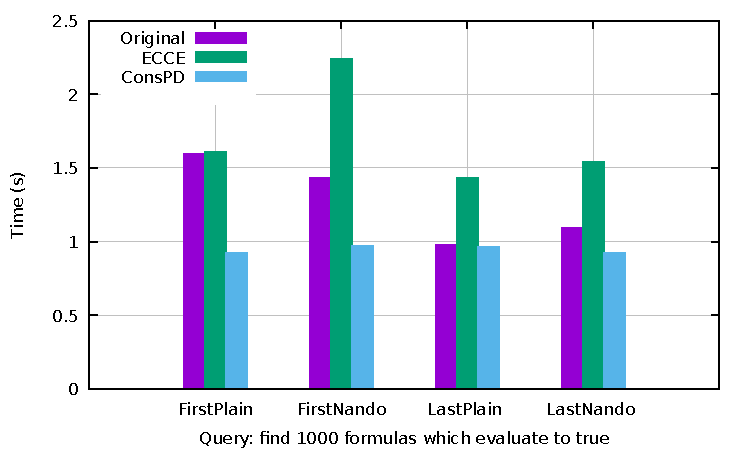
\includegraphics[width=0.45\textwidth]{fig/prop/prop.pdf}
\end{center}
\end{frame}

\begin{frame}[fragile]
  \frametitle{}

\begin{center}
  \Large Functional Conversion
\end{center}

\end{frame}

\begin{frame}[fragile]
  \frametitle{Functional Conversion}

\tikzset{
    block/.style={
      rectangle, draw, minimum width = 2.5cm, minimum height=1.5cm, align=center
        },
}

\newcommand{\fTo}[2]{
  \draw[-Stealth,thick,color=teal] (#1) -- (#2);
}

\begin{center}
  \begin{tikzpicture}[
    every node/.style = {
        inner sep=0pt
      , shape=rectangle
      }
  ]

      \coordinate (shift) at (2.8,-1.5);  

      \node[block] (relInt) at ($(shift)$) {relational \\ conversion};
      \node[block] (spec) at ($(relInt)+(shift)$) {specialization};
      \node[block] (funCon) at ($(spec)+(shift)$) {functional \\ conversion};

      \node[] (args) at ($(spec.west)!(relInt.south)!(spec.east)$) {args};
      \node[] (dir) at ($(funCon.west)!(spec.south)!(funCon.east)$) {direction};

      \node[] (p_m) at ($(relInt.west)!(spec.north)!(relInt.east)$) {p$^o$};
      \node[] (p_i) at ($(spec.west)!(funCon.north)!(spec.east)$) {p$^s$};

      \node[] (p) at ($(relInt.west)+(-0.6,0)$) {$p$};
    
      \node[anchor=west] (haskell) at ($(funCon.north east)+(1,0)$) {Haskell};
      \node[anchor=west] (ocaml) at ($(funCon.east)+(1,0)$) {OCaml};
      \node[anchor=west] (dots) at ($(funCon.south east)+(1,0)$) { $\ \dots$};

      \fTo{$(relInt.east)$}{p_m};
      \fTo{p_m}{spec.north};

      \fTo{$(spec.east)$}{p_i};
      \fTo{p_i}{funCon.north};

      \fTo{p}{$(relInt.west)$};

      \fTo{args}{$(spec.west)$};

      \fTo{dir}{$(funCon.west)$};


      \fTo{funCon.east}{$(haskell.west)$};
      \fTo{funCon.east}{$(ocaml.west)$};
      \fTo{funCon.east}{$(dots.west)$};

  \end{tikzpicture}
  \end{center}
  
  


\end{frame}


\begin{frame}[fragile]
  \frametitle{Example: Addition in the Forward Direction}
\begin{columns}
  \begin{column}[t]{0.49\textwidth}
    \begin{figure}[!t]
  \centering
  \begin{minipage}{0.7\columnwidth}
    \begin{lstlisting}[frame=tb]
 let rec add$^o$ x y z = conde [
   (x === O /\ y === z);
   (fresh (x$_1$ z$_1$)
     (x === S x$_1$ /\
      add$^o$ x$_1$ y z$_1$ /\
      z === S z$_1$) ) ]
    \end{lstlisting}
  \end{minipage}
\end{figure}
    \[ \text{add}^{\circ}\ 0\ 1\ z = \{z \mapsto 1\}\]
  \end{column}
  \begin{column}[t]{0.49\textwidth}
    \begin{figure}[!t]
  \centering
  \begin{minipage}{\columnwidth}
    \begin{lstlisting}[frame=tb]
addIIO :: Nat -> Nat -> Nat
addIIO x y =
  case x of
    O -> y
    S x$_1$ -> S (addIIO x$_1$ y)
    \end{lstlisting}
  \end{minipage}
\end{figure}

    \[ \text{addIIO}\ 0\ 1 = 1 \] 
  \end{column}
\end{columns}
\end{frame}


\begin{frame}[fragile]
  \frametitle{Addition in the Backward Direction: Nondeterminism}
\begin{columns}
  \begin{column}[t]{0.49\textwidth}
    \begin{figure}[!t]
  \centering
  \begin{minipage}{0.7\columnwidth}
    \begin{lstlisting}[frame=tb]
 let rec add$^o$ x y z = conde [
   (x === O /\ y === z);
   (fresh (x$_1$ z$_1$)
     (x === S x$_1$ /\
      add$^o$ x$_1$ y z$_1$ /\
      z === S z$_1$) ) ]
    \end{lstlisting}
  \end{minipage}
\end{figure}
  \end{column}
  \begin{column}[t]{0.49\textwidth}
    \begin{figure}[!t]
  \centering
  \begin{minipage}{0.9\columnwidth}
    \begin{lstlisting}[frame=tb,language=ocanren1]
addOOI $::$ Nat -> Stream (Nat, Nat)
addOOI z =
  return (O, z) <$\mid$>
  case z of
    O -> Empty
    S z$_1$ -> do
      (x$_1$, y) <- addOOI z$_1$
      return (S x$_1$, y)
    \end{lstlisting}
  \end{minipage}
\end{figure}

  \end{column}
\end{columns}

\vfill
$\text{add}^{\circ}\ x\ y\ 1 = \left[\{x \mapsto  0, y \mapsto  1\}, \{x \mapsto  1, y \mapsto  0\} \right]$

\vfill

\lstinline{addOOI 1 = [(0,1), (1,0)]}

\end{frame}

\begin{frame}[fragile]
  \frametitle{Free Variables in Answers: Generators}
\begin{columns}
  \begin{column}[t]{0.49\textwidth}
    \begin{figure}[!t]
  \centering
  \begin{minipage}{0.7\columnwidth}
    \begin{lstlisting}[frame=tb]
 let rec add$^o$ x y z = conde [
   (x === O /\ y === z);
   (fresh (x$_1$ z$_1$)
     (x === S x$_1$ /\
      add$^o$ x$_1$ y z$_1$ /\
      z === S z$_1$) ) ]
    \end{lstlisting}
  \end{minipage}
\end{figure}

    \vspace{0.5cm}
    $\text{add}^{\circ}\ 1\ y\ z = \{z \mapsto S\ y\}$

    \vspace{0.5cm}

    \lstinline{genNat = [0, 1, 2, ...]}

    \vspace{0.5cm}

    \lstinline{addIOO 1 = [(0,1), (1,2), (2,3), ...]} 
  \end{column}
  \begin{column}[t]{0.49\textwidth}
    \begin{figure}[!t]
  \centering
  \begin{minipage}{\columnwidth}
    \begin{lstlisting}[label={add_x},
                      %  caption={Function for \lstinline{addo in out out} direction},
                       captionpos=b,
                       frame=tb]
addX :: Nat -> Stream (Nat, Nat)
addX x = case x of
           O -> do
             z <- genNat
             return (z, z)
           S x' -> do
             (y, z') <- addX x'
             return (y, S z')

genNat :: Stream Nat
genNat = Mature O (S <$\$$> genNat)
    \end{lstlisting}
  \end{minipage}
\end{figure}
  \end{column}
\end{columns}
\end{frame}


\begin{frame}[fragile]
  \frametitle{Modes: Data Flow}
\begin{center}

\begin{tabular}{rl}
    \emph{Ground} term & \lstinline|S (S O)| \\
  \emph{Free} variable & \lstinline|x|
\end{tabular}

\vfill

Once a variable is \emph{ground}, it stays \emph{ground}
\end{center}

\vfill

\begin{center}
\[ \text{Mode} : \text{Inst} \mapsto \text{Inst} \] 
\vfill

\begin{tabular}{rl}
  Mode \lstinline|I|: & \lstinline|ground| $\rightarrow$ \lstinline|ground| \\
  Mode \lstinline|O|: & \lstinline|free| $\rightarrow$ \lstinline|ground|
\end{tabular}
\end{center}

\end{frame}

\begin{frame}[fragile]
  \frametitle{Modded Unification Types}

\begin{center}
\begin{tabular}{rl}
  assignment & $x^{\outmode} \equiv \Term^{\inmode} $ \\
  guard      & $x^{\inmode}  \equiv \Term^{\inmode} $ \\
  match      & $x^{\inmode}  \equiv \Term           $ \\
  generator  & $x^{\outmode} \equiv \Term           $
\end{tabular}
\end{center}

\end{frame}

\begin{frame}[fragile]
  \frametitle{Order in Conjunctions}
\definecolor{badRed}{RGB}{225,0,0}
\definecolor{darkFastGreen}{RGB}{10,46,54}

\newcommand{\badBadge}[1]
{
  \begin{tikzpicture}
    \node[circle,
          scale=0.8,
          text width=1cm,
          fill=badRed,
          draw=darkFastGreen,
          line width=0.4mm,
          inner sep=1pt,
          align=center]
        {\textbf{#1}};
  \end{tikzpicture}
}

\definecolor{fastGreen}{RGB}{41,231,204}
\definecolor{darkFastGreen}{RGB}{10,46,54}

\newcommand{\goodBadge}[1]
{
  \begin{tikzpicture}
    \node[circle,
          scale=0.8,
          text width=1cm,
          fill=fastGreen,
          draw=darkFastGreen,
          line width=0.4mm,
          inner sep=1pt,
          align=center]
        {\textbf{#1}};
  \end{tikzpicture}
}
\lstset{language=ocanren1,basicstyle={\ttfamily \footnotesize}}

\begin{center}
  \begin{tikzpicture}[
    every node/.style = {
        inner sep=0pt
      , shape=rectangle
      % , draw
      }
  ]
      % \draw[help lines] (-7.75,-3.5) grid (7.75,3.5);
      \node[inner sep=10pt, anchor=north west] (func) at (-7.75,3.5) {\begin{minipage}{0.35\columnwidth}
  \begin{lstlisting}[frame=tb]
 let rec mult$^o$ x y z = conde [
   (fresh (x$_1$ r$_1$)
     (x === S x$_1$) /\
     (add$^o$ y r$_1$ z) /\
     (mult$^o$ x$_1$ y r$_1$));
   ...]
\end{lstlisting}
\end{minipage}};

      \node[inner sep=10pt, anchor=north east] (slow) at (7.75,3.5) {\begin{minipage}{0.52\columnwidth}
  \begin{lstlisting}[frame=tb]
 multIIO$_1$ $::$ Nat -> Nat -> Stream Nat
 multIIO$_1$ (S x$_1$) y    = do
   (r$_1$, r) <- addIOO y
   multIII x$_1$ y r$_1$
   return r
 ...
 multIII $::$ Nat -> Nat -> Nat -> Stream ()
 multIII (S x$_1$) y z = do
   z$_1$ <- multIIO$_1$ x$_1$ y
   addIII y z$_1$ z
 multIII _ _ _ = Empty
 ...
\end{lstlisting}
\end{minipage}
};

      \node [draw=none, above=of slow.south, xshift=2.3cm] {\badBadge{$\Omega(x!)$}};

      \node[ellipse, scale=0.8,
          fill=badRed!75,
          draw=darkFastGreen,
          line width=0.4mm,
          inner sep=1pt,
          align=center, above=of slow.south, xshift=2.5cm, yshift=4cm]
        {\textbf{generate-and-test}};

      \node[inner sep=10pt, anchor=south west] (fast) at (-7.75,-3.5) {\begin{minipage}{0.42\columnwidth}
\begin{lstlisting}[frame=tb]
multIIO $::$ Nat -> Nat -> Stream Nat
multIIO (S x$_1$) y = do
  r$_1$ <- multIIO x$_1$ y
  addIIO y r$_1$
...
\end{lstlisting}
\end{minipage}
};

      \node [draw=none, anchor=south west] at ($(fast.south)+(0.5,0.8)$) {\goodBadge{$O(xy)$}};
      \node [draw=none, above=of fast.south, xshift=2.3cm] {\goodBadge{10x \linebreak faster}};
  \end{tikzpicture}
  \end{center}
  
\end{frame}

\begin{frame}[fragile]
  \frametitle{Mode Inference: Ordering Heuristic}

\begin{center}
  \begin{minipage}{0.4\textwidth}
    \begin{enumerate}
      \item Guard
      \item Assignment
      \item Match
      \item Recursion, same direction
      \item Call, some args ground
      \item Unification-generator
      \item Call, all args free
    \end{enumerate}
  \end{minipage}
\end{center}


\end{frame}

\begin{frame}[fragile]
  \frametitle{Ordering Heuristic: Example}
\begin{center}
  \begin{tikzpicture}[
    every node/.style = {
        inner sep=0pt
      , shape=rectangle
      % , draw
      }
  ]
      % \draw[help lines] (-7.75,-3.5) grid (7.75,3.5);
      \node[inner sep=10pt, anchor=north] (func) at (-7.75,3.5) {\begin{minipage}{0.35\columnwidth}
  \begin{lstlisting}[frame=tb]
 let rec mult$^o$ x y z = conde [
   (fresh (x$_1$ r$_1$)
     (x === S x$_1$) /\
     (add$^o$ y r$_1$ z) /\
     (mult$^o$ x$_1$ y r$_1$));
   ...]
\end{lstlisting}
\end{minipage}};

      \node[inner sep=10pt, anchor=south] (fast) at (-7.75,-3.5) {\begin{minipage}{0.42\columnwidth}
\begin{lstlisting}[frame=tb]
multIIO $::$ Nat -> Nat -> Stream Nat
multIIO (S x$_1$) y = do
  r$_1$ <- multIIO x$_1$ y
  addIIO y r$_1$
...
\end{lstlisting}
\end{minipage}
};

  \end{tikzpicture}
  \end{center}
  

\end{frame}


\begin{frame}[fragile]
  \frametitle{Relational Sort}
\begin{columns}
  \begin{column}[t]{0.49\textwidth}
    
\lstset{moredelim=[is][\bfseries]{[*}{*]}}

\begin{figure}[h]
  \centering
  \begin{minipage}{0.65\columnwidth}
    \begin{lstlisting}[frame=tb,language=ocanren1]
 let rec sort$^o$ x y =
   (x === [] /\ y === []) \/ 
   (fresh (s xs xs$_1$)
     y === s :: xs$_1$ /\
     smallest$^o$ x s xs /\
     sort$^o$ xs xs$_1$)
    \end{lstlisting}
  \end{minipage}
\end{figure}


    \vfill

    \begin{center}
      \begin{minipage}{0.4\textwidth}
        \begin{itemize}
          \item[\happyCheck] sorting
          \item[\timeout] permutations
        \end{itemize}
      \end{minipage}
    \end{center}

  \end{column}
  \begin{column}[t]{0.49\textwidth}
    \begin{figure}[h]
  \centering
  \begin{minipage}{0.87\columnwidth}
    \begin{lstlisting}[frame=tb]
 let rec sort$^o$ x y = conde [
    (x === [] /\ y === []);
    (fresh (s xs xs$_1$)
      y === s :: xs$_1$ /\
      [*sort$^o$ xs xs$_1$ /\
      smallest$^o$ x s xs)*]]
    \end{lstlisting}
  \end{minipage}
\end{figure}
 

    \vfill

    \begin{center}
      \begin{minipage}{0.4\textwidth}
        \begin{itemize}
          \item[\timeout] sorting
          \item[\happyCheck] permutations
        \end{itemize}
      \end{minipage}
    \end{center}


  \end{column}
\end{columns}
\end{frame}


\begin{frame}[fragile]
  \frametitle{Relational Sort: Sorting}
    \begin{table}[]
\begin{tabular}{l||c|r||r}
                & \multicolumn{2}{c||}{Relation} & \multicolumn{1}{c}{\multirow[t]{2}{*}{Function}} \\ \cline{2-3}
                & \multicolumn{1}{l|}{\begin{tabular}[c]{@{}l@{}}\texttt{sorto}\\ \texttt{smallesto}\end{tabular}} & \multicolumn{1}{l||}{\begin{tabular}[c]{@{}l@{}}\texttt{smallesto}\\ \text{sorto}\end{tabular}} & \multicolumn{1}{c}{}                            \\ \hline
\texttt{{[}3;2;1;0{]}}   & \multicolumn{1}{r|}{0.077s}                                                    & 0.004s                                                                         & 0.000s                                          \\
\texttt{{[}4;3;2;1;0{]}} & \timeout timeout                                                                       & 0.005s                                                                         & 0.000s                                          \\
\texttt{{[}31;...;0{]}}  & \timeout timeout                                                                       & 1.058s                                                                         & 0.006s                                          \\
\texttt{{[}262;...;0{]}} & \timeout timeout                                                                       & \multicolumn{1}{c||}{\timeout timeout}                                                   & 1.045s
\end{tabular}
\end{table}


\end{frame}


\begin{frame}[fragile]
  \frametitle{Relational Sort: Generating Permutations}
    \begin{table}[]
\begin{tabular}{l||c|r||r}
                & \multicolumn{2}{c||}{Relation} & \multicolumn{1}{c}{\multirow[t]{2}{*}{Function}} \\ \cline{2-3}
                & \multicolumn{1}{l|}{\begin{tabular}[c]{@{}l@{}}\texttt{smallesto}\\ \texttt{sorto}\end{tabular}} & \multicolumn{1}{l||}{\begin{tabular}[c]{@{}l@{}}\texttt{sorto}\\ \text{smallesto}\end{tabular}} & \multicolumn{1}{c}{}                            \\ \hline
\texttt{{[}0;1;2{]}}   & \multicolumn{1}{r|}{0.013s}                                                    & 0.004s                                                                         & 0.004s                                          \\
\texttt{{[}0;1;2;3{]}} & \timeout timeout                                                                       & 0.005s                                                                         & 0.005s                                          \\
\texttt{{[}0;...;6{]}}  & \timeout timeout                                                                       & 0.999s                                                                         & 0.021s                                          \\
\texttt{{[}0;...;8{]}} & \timeout timeout                                                                       & \multicolumn{1}{c||}{\timeout timeout}                                                   & 1.543s
\end{tabular}
\end{table}

\end{frame}


\begin{frame}[fragile]
  \frametitle{\lstinline[basicstyle=\Large]{Maybe} for Semi-Determinism}
\begin{center}
  \begin{minipage}{0.5\textwidth}
    \begin{center}
  \begin{tikzpicture}[
    every node/.style = {
      shape=rectangle,
      rounded corners=0.05cm,
      draw,
      align=center,
      minimum size=5mm},
    node distance=1.3em,
    anchor=center
  ]
    \node[inner sep=10pt,draw=none] (code) at (0,0) {
      \begin{minipage}{\columnwidth}
      \begin{lstlisting}[]

 ~\texttt{muloOII $::$ Nat $\to$ Nat $\to$ Stream Nat}~
 muloOII x1 x2 =
     zero <$\mid$> positive
   where
     zero = do
       guard (x2 == O)
       return O
     positive = do
       x4 <- addoIOI x1 x2
       S <$\$$> muloOII x1 x4
       \end{lstlisting}
      \end{minipage}
    };
  \end{tikzpicture}
  \end{center}
  
    % \begin{figure}[!t]
  \centering
  \begin{minipage}{\columnwidth}
    \begin{lstlisting}[frame=tb]
muloOII :: Nat -> Nat -> Stream Nat
muloOII x1 x2 = zero `mplus` positive
  where
    zero = do
      guard (x2 == O)
      return O
    positive = do
      x4 <- addoIOI x1 x2
      S <$\$$> muloOII x1 x4
    \end{lstlisting}
  \end{minipage}
\end{figure}
  \end{minipage}
\end{center}
\end{frame}

\begin{frame}[noframenumbering]
  \frametitle{\lstinline[basicstyle=\Large]{Maybe} for Semi-Determinism}
  \begin{center}
  \begin{minipage}{0.5\textwidth}
    \begin{center}
  \begin{tikzpicture}[
    every node/.style = {
      shape=rectangle,
      rounded corners=0.05cm,
      draw,
      align=center,
      minimum size=5mm},
    node distance=1.3em,
    anchor=center
  ]
    \node[inner sep=10pt,draw=none] (code) at (0,0) {
      \begin{minipage}{\columnwidth}
      \begin{lstlisting}[]
 ~\texttt{muloIIO $::$ Nat $\to$ Nat $\to$ Maybe Nat}~
 ~\lststrikethrough{muloIIO $::$ Nat $\to$ Nat $\to$ Stream Nat}~
 muloIIO x y =
     zero <$\mid$> positive
   where
     zero = do
       guard (x == O)
       return O
     positive = do
       (S $x_1$) <- return x
       $z_1$ <- muloIIO $x_1$ y
       z <- addoIIO $z_1$ y
       return z
       \end{lstlisting}
      \end{minipage}
    };
    \node [draw=none, above=of code.south, xshift=2.5cm, yshift=2.5cm] {\goodBadge{10x \linebreak faster}};
  \end{tikzpicture}
  \end{center}
  

    % \lstset{moredelim=[is][\sout]{|}{|}}

\begin{figure}[!t]
  \centering
  \begin{minipage}{\columnwidth}
    \begin{lstlisting}[]
 ~\texttt{muloOII $::$ Nat $\to$ Nat $\to$ Maybe Nat}~
 ~\lststrikethrough{muloOII $::$ Nat $\to$ Nat $\to$ Stream Nat}~
 muloOII x1 x2 =
     zero <$\mid$> positive
   where
     zero = do
       guard (x2 == O)
       return O
     positive = do
       x4 <- addoIOI x1 x2
       S <$\$$> muloOII x1 x4
    \end{lstlisting}
  \end{minipage}
\end{figure}

  \end{minipage}
\end{center}
\end{frame}


\begin{frame}[fragile]
  \frametitle{Conclusion}

\begin{itemize}
  \item We created a specialization method for \mk
  \item We implemented a functional conversion scheme
  \item They both speed up implementations considerably
\end{itemize}
\end{frame}

\end{document}
